\documentclass[11pt,nswissgerman]{article}
\usepackage{helvet}
\renewcommand{\familydefault}{\sfdefault}
\usepackage[utf8x]{inputenc}
\usepackage[a4paper]{geometry}
\geometry{verbose,tmargin=3cm,bmargin=3cm,lmargin=3.5cm,rmargin=3.5cm,headheight=3cm,headsep=1cm,footskip=2cm}
\usepackage{fancyhdr}
\pagestyle{fancy}
\usepackage{wrapfig}
\usepackage{graphicx}
\usepackage[position=bottom]{subfig}
\usepackage{titletoc}
\usepackage{float}
\makeatletter
\@ifundefined{date}{}{\date{}}
\makeatother
\usepackage{babel}
\usepackage[
            colorlinks=true,
            urlcolor=green,
            linkcolor=black
]{hyperref}
\setcounter{secnumdepth}{1} % levels under \section are not numbered
\setcounter{tocdepth}{2}    % levels under \subsection are not listed in the TOC
\begin{document}
\author{Stefan Bopp}
\title{\Huge Sommer 2012 Italien / Kroatien \\[2cm]

\includegraphics[width=0.4\textwidth]{../Bilder/Logo/Logo.png}
}
\maketitle
\vfill
\tableofcontents

\newpage

\lhead{Sommer 2012}

\rhead{jackthebus.com}

\cfoot{\thepage}
\subsection{31.07.2012 Die letzten Vorbereitungen}
Da unsere n�rdlichen Nachbarn mit der Lieferung von sehnlichst erwarteten Ersatzteilen in Verzug waren, musste unser Notnagel Tobi einspringen.
Zuverl�ssig wie eh und je konnte ich am Abend die ben�tigten Teile abholen.
Das Ganze noch Kurz im Bus eingebaut und der langen Fahrt sollte nichts mehr im Wege stehen.
Die Batterie, welche in letzter Zeit eher mit schwacher Leistung gegl�nzt hatte, konnte dank Garantie problemlos eingetauscht werden. (Danke Chantal)

\subsection{01.08.2012 Nutzlast?}
Der Tag stand ganz im Zeichen der Nahrungsaufnahme.
Der aufmerksame Beobachter k�nnte meinen, dass wir unsere K�rpereigenen Reserven f�r unsere Reise aufladen.
Jedoch war der Grund nicht die Angst vor einer drohenden Hungersnot, sonder der 1.August, Nationalfeiertag der Schweiz.
Also reingehauen, kann ja nicht schaden.
Trotzdem mussten die anstehenden Arbeiten noch erledigen werden.
Das Tanken kurz nach dem traditionellen Feuerwerk in Baden bescherte der Coop-Tankstelle einen fetten Benzinflecken.
Mein �bermut und meine Viel hilft viel Philosophie wurde bestraft.
Der �bergang von Tankstutzen zu Benzintank pr�sentiert sich leicht spr�de und der wertvolle Saft fand den Weg aus dem Bus zur�ck zur Tankstelle.
Gl�cklicherweise befindet sich das Leck in naher Distanz zum Tankdeckel.
So kam es, dass wir erst nach 11 Uhr unser wohlverdienter Sch�nheitsschlaf beginnen konnten.
Schon arg nahe am unsch�nen Weckerton, welcher uns um 04:30 f�r den Beginn der Reise aus den Federn holen sollte. 
Als erstes Ziel wollten wir m�glichst viele Kilometer hinter uns bringen, damit wir nicht jeden Tag Auto fahren m�ssen.
Unser zugegebenerma�en ambiti�se Ziel war: Rom.
Viele Wege f�hren nach Rom, doch wir werden nur einen ben�tigen.
Viele selbsternannte Kritiker und M�chtegern VW-Bus Kenner l�chelten �ber unser Vorhaben und streuten gezielt Zweifel.
Auch wir waren nach den j�ngsten Ereignissen nicht abgeneigt den allj�hrlichen TCS Beitrag zu bezahlen um f�r das allerschlimmste gewappnet zu sein.  

\begin{figure}[hbt]
    \centering
    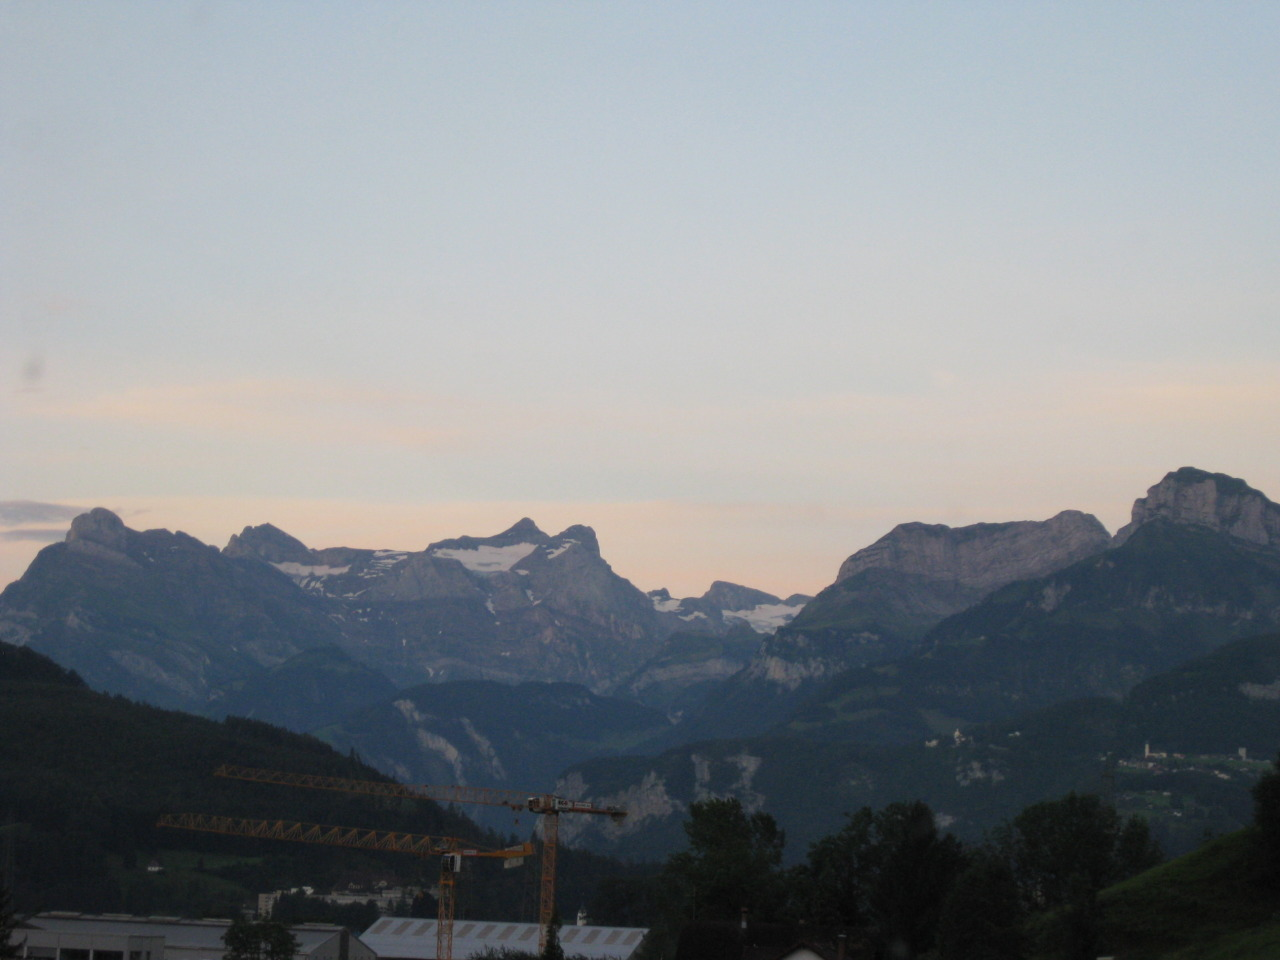
\includegraphics[width=\textwidth]{../Bilder/Sommer2012/1.jpg}
    \caption{Auf dem Weg in den S�den}
    \label{img:Sommer1}
\end{figure}

\subsection{02.08.2012 Es geht los}
Kurz nach 5 Uhr waren auch die letzten Ausreden, welche gegen eine Abfahrt gesprochen h�tten aus dem Weg ger�umt und wir machten uns auf den Weg gen S�den.
Schon fr�h fanden wir einen geeigneten LKW um uns in den Windschatten zu h�ngen und die Reise bei einem geringerem L�rmpegel zu absolvieren.
Der Berufsverkehr hielt sich in Grenzen und schon bald konnten wir unseren ersten Espresso an der Rastst�tte Gottardo Sud genie�en.
Kurz nach der ersten Pause wurde die Frage nach dem Fackel f�r die F�hr�berfahrt nach Kroatien leider negativ beantwortet.
Eine wilde Suche nach dem Best�tigungsmail auf dem Handy begann.
Wir entschlossen uns die n�chste Rastst�tte zu nutzen um mittels Laptop nach dem vermeintlich verloren gegangenen Mail zu suchen.
Die Suche f�hrte zu einem Treffer im SPAM Ordner, welcher einen Tag sp�ter automatisch gel�scht worden w�re.
Gl�ck gehabt. Weiter ging die Reise Richtung Italienischer Grenze.

Da Jack mittlerweile zum Liebling der Polizeikontrollen avanciert ist (Sind daran m�glicherweise die gr�nen Hibiskusbl�ten schuld?), waren wir auf den Grenz�bertritt gespannt.
Doch ganz im Stile echter Italienischer Staatsangestellten verbrachten die anwesenden Z�llner ihre Zeit lieber mit Sp�sse als mit Kontrollen.

Nach einer kurzen Phase der Verkehrs�berlastung um Mailand ging die Flotte Reise Richtung S�den ungebremst weiter.
Die Landschaft wurde viel zu selten durch interessante Aussichten gest�rt.
Dominierend waren Felder und Hochspannungsmasten.
Waren zu Beginn die Temperaturen noch angenehm, n�herte sich das Thermometer je l�nger je n�her der Zone ziemlich bis wahnsinnig warm.
Man konnte H�hnchen fettarm zubereiten, wenn man sie aus dem offenen Fenster h�lt.
Gerade in Mitten einer LKW Kolonne, welche sehr h�ufig (zu h�ufig) auftraten, war der Atem eines Heissluftf�hnes zu sp�ren.
Die lieben Lkws machten Chantal zu schaffen.
Gerade als sie den n�tigen Schwung f�r ein �berholman�ver gesammelt hatte, scherte der schl�frige Chauffeur mit seinem langen Gef�hrt Richtung unserer Spur.
Dieses Man�ver provozierte eine wahre Sammlung netter Ausdr�cke, welche in ihrer Rohform so im �ffentlichen Raum nicht abgedruckt werden sollten.

Endlich n�herten wir uns Rom und damit begann die Suche nach einer Bleibe.
Die elektronische Sammlung von Campingpl�tzen um Rom schlug uns zwei Favoriten vor.
Um �berhaupt dort hin zu kommen mussten wir den Westring von Rom befahren, welcher uns mit Stau und den dazugeh�rigen spannenden �berholman�ver begr��te.
Der erste Angesteuerte Campingplatz war closed.
So jedenfalls die Aussage eines beim Eingang abgestellten Typen.
Wir sollen es bei einem anderen Versuchen.
Das taten wir und wir hatten Gl�ck.
200 Meter vom Strand entfernt fanden wir kurz vor 19:00 unser erster Standplatz.
Nach dem hastigen Einrichten stand einem Bad im Meer nichts mehr im Weg.

Auf dem R�ckweg sahen wir ein sch�ne Restaurant am Meer, welches aber alles andere als gut besucht war.
Wir beschlossen, unser Gl�ck nach dem Frischmachen dort zu suchen.
Nat�rlich war um 22:00 das lokal von Einheimischen �bersp�lt worden.
Ein kurzer Blick �ber die Strandpromenade bescherte uns Gewissheit, dass dieses Lokal das einzig brauchbare zu sein scheint.
Nur hier waren Autos geparkt.
So mussten wir uns mit dem Campingrestaurant begn�gen.
Wir wurden keinesfalls Entt�uscht.
Chantal stellte die Spaghetti Pesto in Rekordzeit herunter und auch ich musste mich keinesfalls hinter der Pizza verstecken.
Die eigentlich ganz fleissige Bedienung musste jedoch genau in der Phase, in der die M�cken wieder ein prominentes Opfer gefunden haben, eine, nein zwei Rauchpausen einlegen.
Kurz vor 24:00 war der erste lange Tag unserer Reise Geschichte.

\begin{figure}[h]
   \centering
      %\subfloat[CAPTION]{BILDERCODE}\qquad
   \subfloat{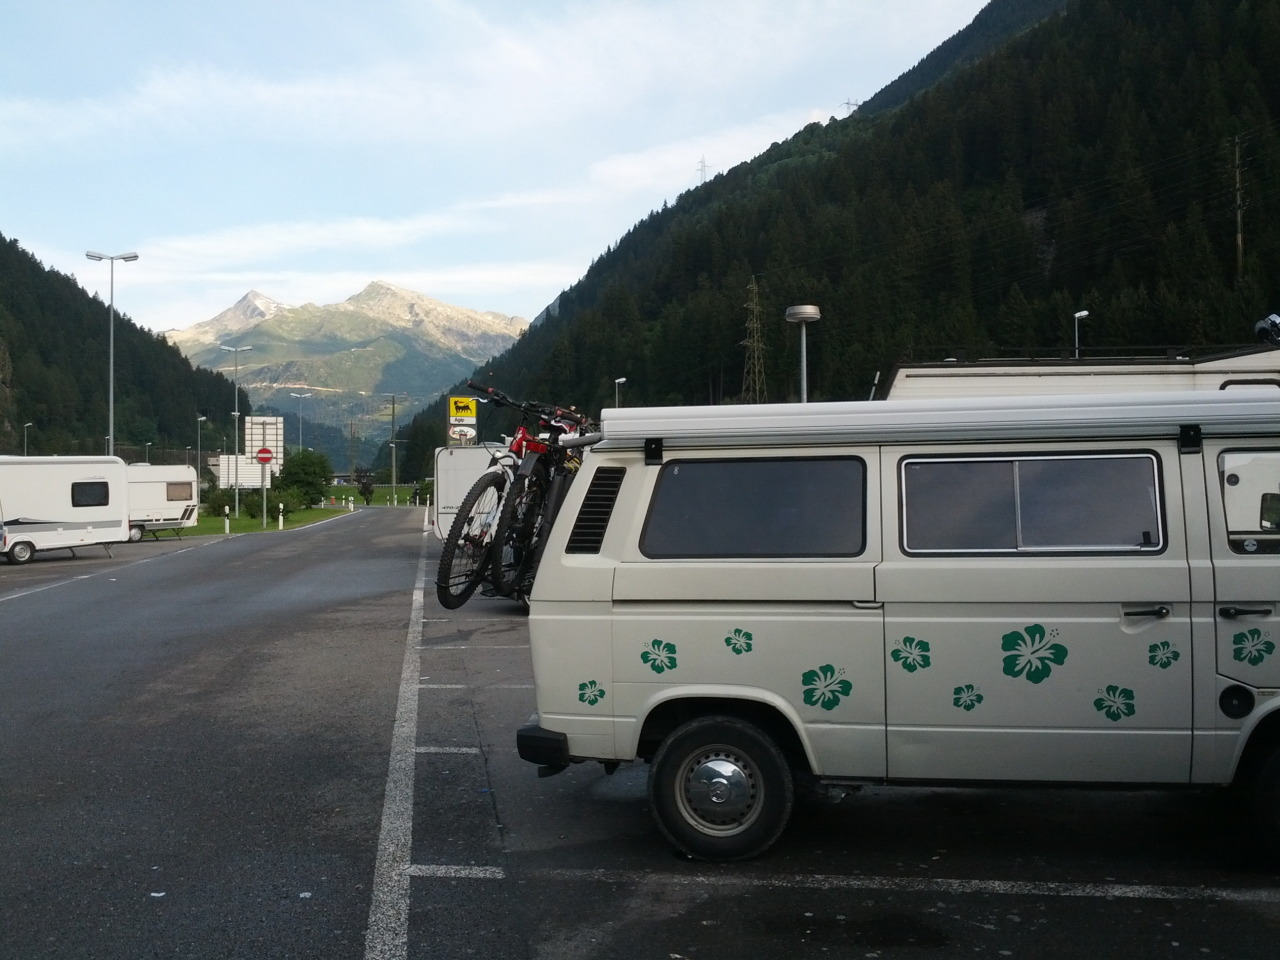
\includegraphics [width=0.3\textwidth]{../Bilder/Sommer2012/2.jpg}}\quad
   \subfloat{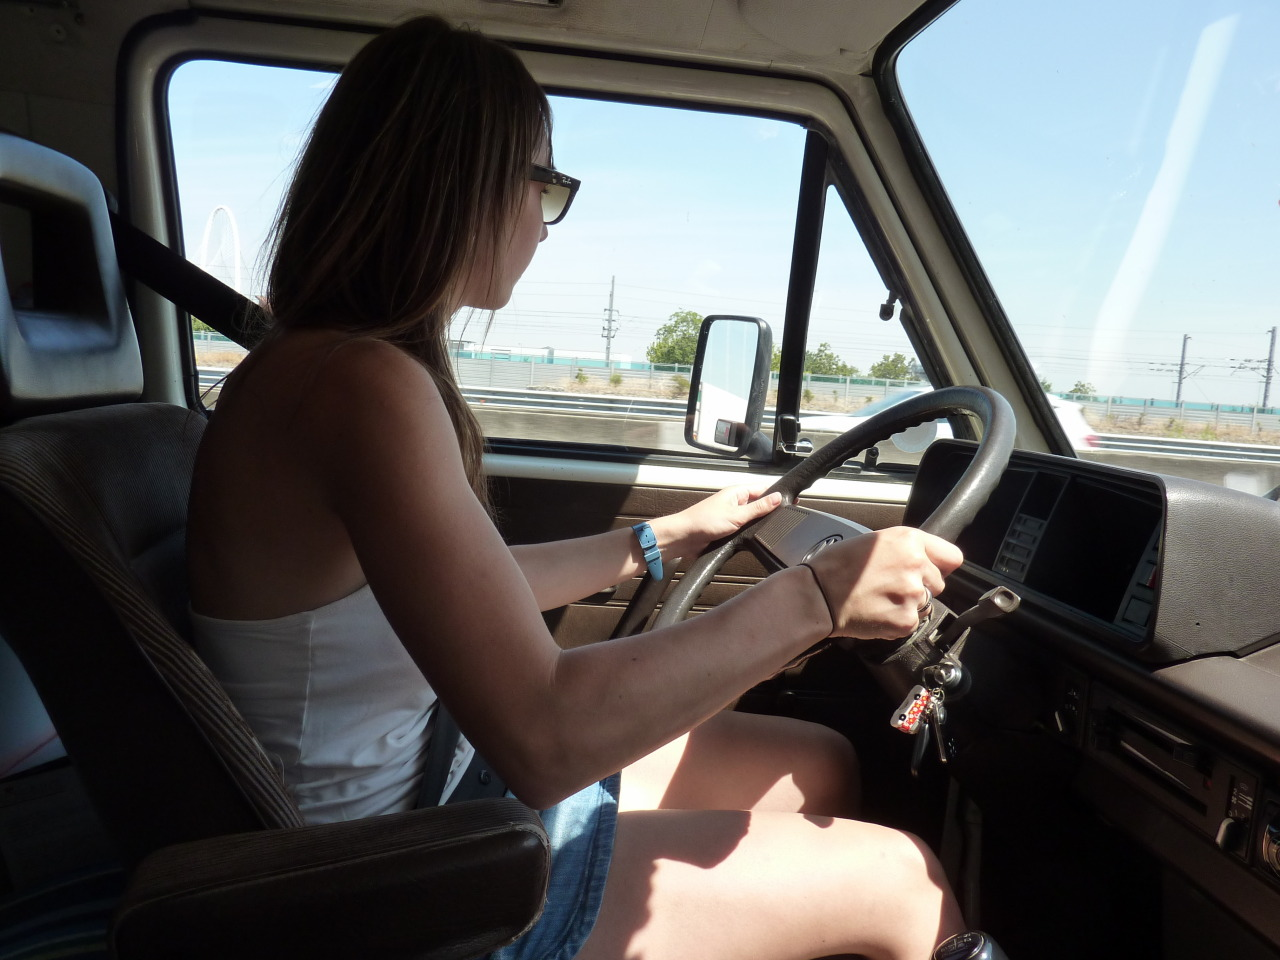
\includegraphics [width=0.3\textwidth]{../Bilder/Sommer2012/3.jpg}}\quad
   \subfloat{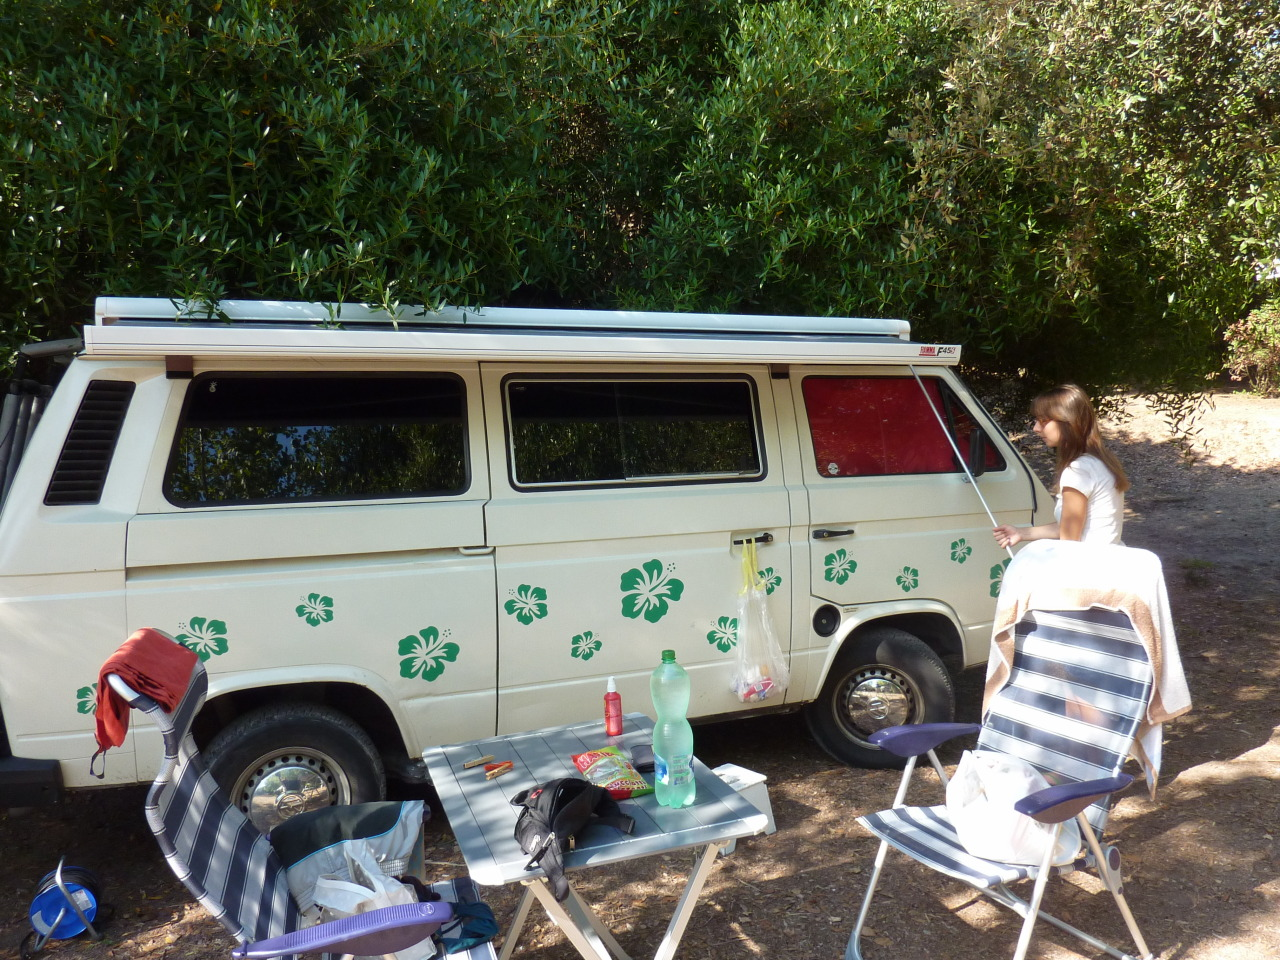
\includegraphics [width=0.3\textwidth]{../Bilder/Sommer2012/5.jpg}}\quad
   \caption[Weg und Ankunft in Rom]{Weg und Ankunft in Rom}
\end{figure}

\subsection{03.08.2012 Roma bei gef�hlten 220� C}
Durch die geschickte Platzwahl konnten wir wunderbar im Schatten aufwachen.
Die Temperaturen waren auf ein angenehmes Mass gesunken w�hrend der Nacht.
Doch was bewegt sich da? AMEISEN.
Nicht gerade wenige nutzten unseren Bus als eine Art �bergrosse Treppe um von einem Baum auf den Boden zu kommen.
Bei dieser Gelegenheit betrachteten diese Biester auch gerade noch unsere Innenraumaustattung.
Frechheit sowas.
Umparken war angesagt.
Mittels wilder Rangierman�ver ohne R�cksicht auf Flora und Fauna war der neue Standplatz inert Minutenfrist erreicht.
Anti-Brumm scheinen die vielbeinigen Plaggeister nicht zu m�gen.
Jedenfalls veranstalten sie bei jedem Spr�hangriff einen wilden Tanz und fallen wie Reife Pflaumen vom Bus.
Das Fr�hst�ck wurde trotzdem genossen.

Nach kurzer Recherche verwarfen wir die verwegene Idee Rom vom Campingplatz aus mit dem Velo zu erkunden.
Weit �ber 25 km Distanz und Aussicht auf einen eher warmen Tag machten uns diese Entscheidung leicht.
�V f�hrt von hier bis ins Stadtzentrum und diese Transportmittel nutzen wir auch um in ca 1 Stunde neben dem Kolosseum aus dem Untergrund in der Hitze aufzutauchen.
Naja, so kolossal sah diese Ruine jetzt nicht gerade aus.
Auch das Forum Roman haute uns nicht aus den Socken oder �hm Sandalen.
Mit R�mersandalen wollte ich durch das Forum Roman schlendern und die Latein-stunden der Bezirksschule wieder aufleben lassen: Ave Ceasar.
.Salve Titus.
.;) aber die Ruinen des Forums sahen gar nicht einladend aus; sie glichen eher einem Friedhof als einer spektakul�ren und historischen St�tte.
So machten wir uns auf den Weg zu der spanischen Treppe, die bekannteste Treppe der Welt.
Aber wo war diese? Obwohl sie ziemlich gross ist, hatten wir M�he sie zu orten.
Da die Geographin die Treppe neben dem Forum Roman vermutete, sie aber �berhaupt nicht dort war, wurde aus jeder Treppe rings um das Forum Roman die spanische Treppe ;) So haben wir viele Treppen erklommen und uns immer gedacht: die ist aber nicht so imposant wie auf dem Bild.
Nach einigen Fehlversuche haben wir dann doch herausgefunden, dass wir auf der falschen F�hrte sind und haben einen neuen Anlauf genommen.

\begin{figure}[h]
   \centering
      %\subfloat[CAPTION]{BILDERCODE}\qquad
   \subfloat{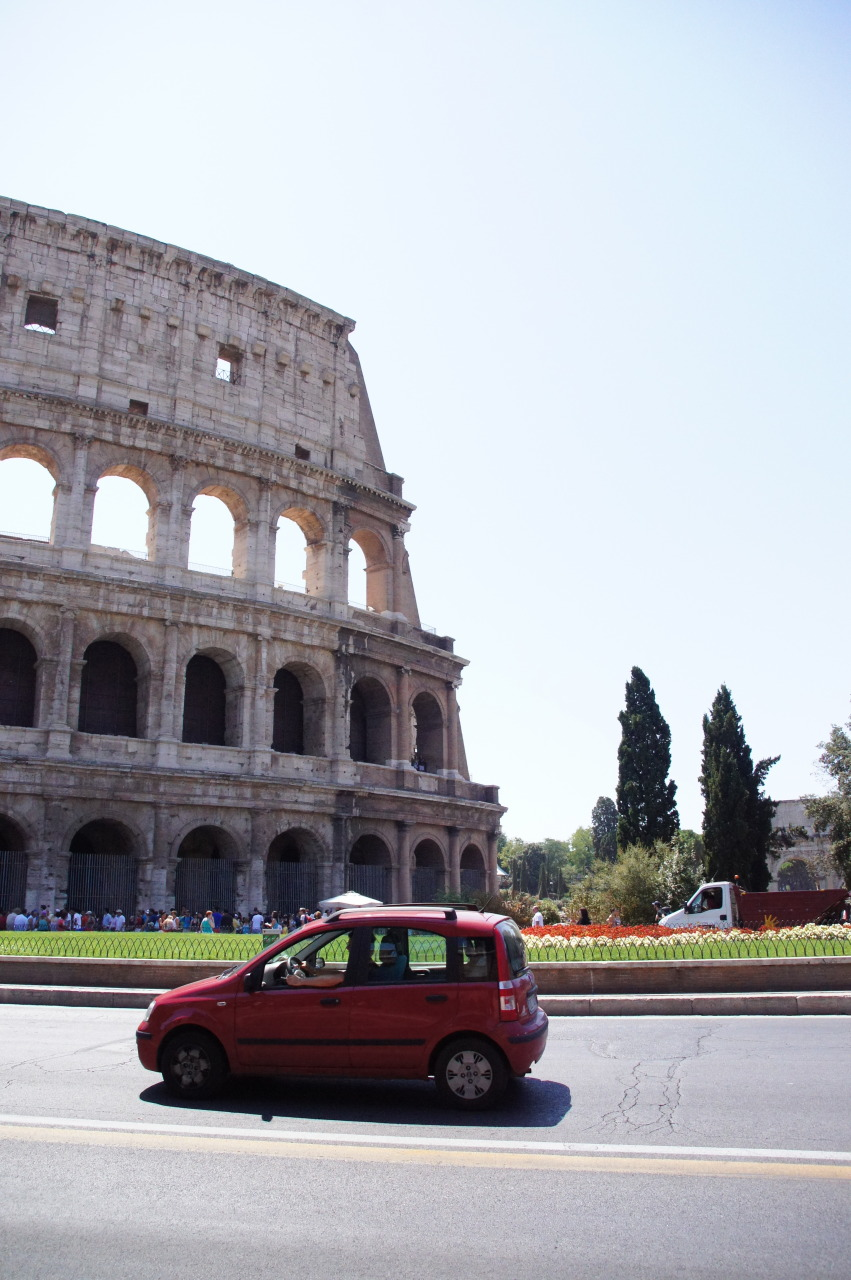
\includegraphics [width=0.3\textwidth]{../Bilder/Sommer2012/6.jpg}}\quad
   \subfloat{
\includegraphics [width=0.3\textwidth]{../Bilder/Sommer2012/7.jpg}}\quad
   \subfloat{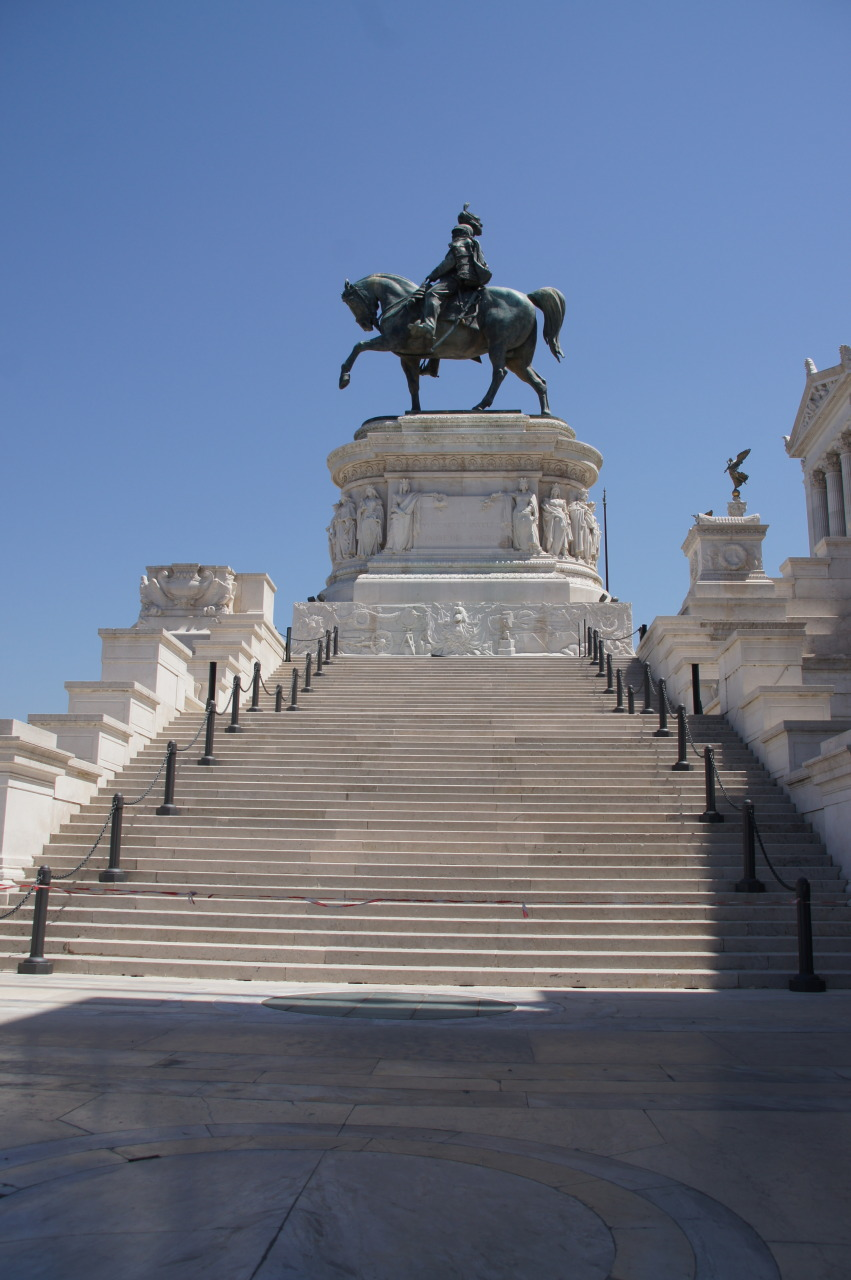
\includegraphics [width=0.3\textwidth]{../Bilder/Sommer2012/8.jpg}}\quad
   \caption[Sightseeing in Rom]{Sightseeing in Rom}
\end{figure}

Und da liefen wir direkt ins Judenviertel; j�dische Touristeninformation, Judensterne und koscher Essen gab es �berall und das direkt neben dem Vatikan.
Sogar koscher Kebab gab es.
Dann meldete sich der Hunger.
Wir g�nnten uns eine Pizza und Bruschetti, was aber eher eine schlechte Idee war.
Von der brennenden Sonne verging uns schnell der Hunger und wir k�mpften um jeden Bissen.
Nur mit viel Wasser und Cola konnten wir fast alles herunterschlingen.
Die Konsequenz daraus war, dass unser Magen bei der Hitze das Essen nicht so gut ertrug und wir uns nach dem Essen schlechter f�hlten als bevor.
Steff k�mpfte mit der Hitze und der Pizza im Magen.
So marschierten wir zur spanischen Treppe, die wir schlussendlich auch fanden und welche immer noch nicht so spektakul�r wie auf dem Bild im Reisef�hrer aussah.
Nach einem Drink (viiiiel Wasser;)) machten wir uns dann auch schon auf den Heimweg.
Wir mussten uns eingestehen, dass ein Stadtbesuch bei dieser Hitze nicht so angenehm ist.
Im Camping angekommen, freuten wir uns auf die Dusche und einen gem�tlichen Abend.
Zum Nachtessen gab es feine Chilli-Oliven, Chips und Tomatensalat.
Mehr vertrug unser gestresste Magen nicht;) Wir lasen vertieft in unseren B�chern mit sch�ner Musik (Campingband) im Hintergrund.

\subsection{04.08.2012 Relaxxxxx}
Dieser Tag stand ganz im Zeichen des Faulenzen.
Wir schliefen aus und auch die aggressiven Ameisen konnten uns nicht fr�her aus den Federn holen.
Danach war ein Tag am Strand angesagt.
Mit Hilfe von Sonnenschirm und Wind konnte es man problemlos einen ganzen Tag am Strand aushalten.
Lesen und Faulenzen...
Am Abend besuchten wir das Restaurant am Strand, welches am ersten Tag hoffnungslos �berlaufen war.
Dieses Mal reservierten wir jedoch.
Die Servierd�se konnte mir alles andrehen, jedenfalls sah das Chantal so und darum wurde aus dem Znacht ein gediegenes Mahl.
Erst sp�t am Abend kehrten wir zu unserem Bus zur�ck wo wir m�de in Federn fallen wollten.
Jedoch machte uns ein hinterlistiges Sandkorn einen Strich durch die Rechnung.
Irgendwie verfing sich dieses Korn in einem Auge und blieb dort hartn�ckig die ganze Nacht, was zu einer eher ungem�tlichen Nacht f�hrte

\begin{figure}[hbp]
    \centering
    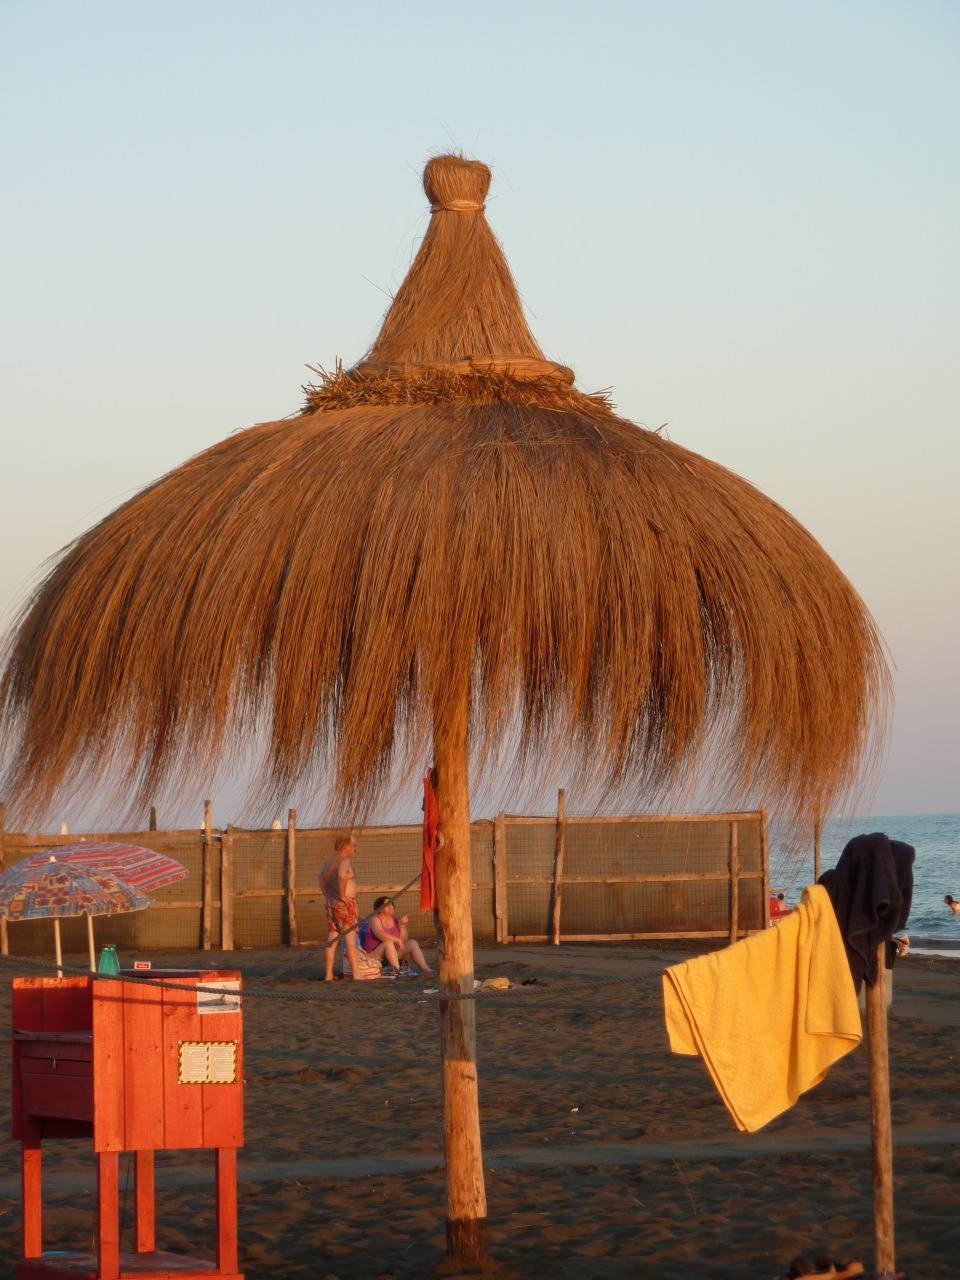
\includegraphics[width=\textwidth]{../Bilder/Sommer2012/4.jpg}
    \caption{Am Strand in Rom}
    \label{img:Sommer2}
\end{figure}

\subsection{05.08.2012 Je s�dlicher ,desto tsch tsch}
Der Morgen kam viel zu fr�h und beide Busfahrer hatten irgendwie einen komischen Magen.
So fiel das Fr�hst�ck sehr sp�rlich aus und schon bald fingen wir an unsere 7 Sachen im Bus zu verstauen.
Um 10 Uhr war Abfahrt und der Weg f�hrte Richtung Vieste.
Es wurde zu einer �u�erst ungem�tlichen Fahrt, welche nur ein gutes Ende nahm, weil gewisse Tabletten aus Armeebest�nde den Weg in unsere M�gen fanden (Besten Dank dem Dr.  Sponsor).
Wir wollten die Fahrt schon aus gesundheitlichen Gr�nden unterbrechen, bissen uns dann aber bis nach Peschici durch.
Auch Jack musste das erste Mal so richtig leiden.
Die Temperatur blieb zwar stets im gr�nen Bereich, jedoch wollte er mit Hilfe des Standgases nicht mehr unbedingt seinen Dienst tun.
Unser neu montiertes Endrohr hing nur noch an einer Schraube statt an deren Drei.
Draht schafft hier Abhilfe (hoffentlich) Auch um 20:00 ist hier das Thermometer noch auf den oberen Etagen unterwegs und denkt nicht einmal daran in angenehmere Regionen zu sinken.
Das wird eine feucht-(fr�hliche) Nacht.

\begin{figure}[H]
    \centering
    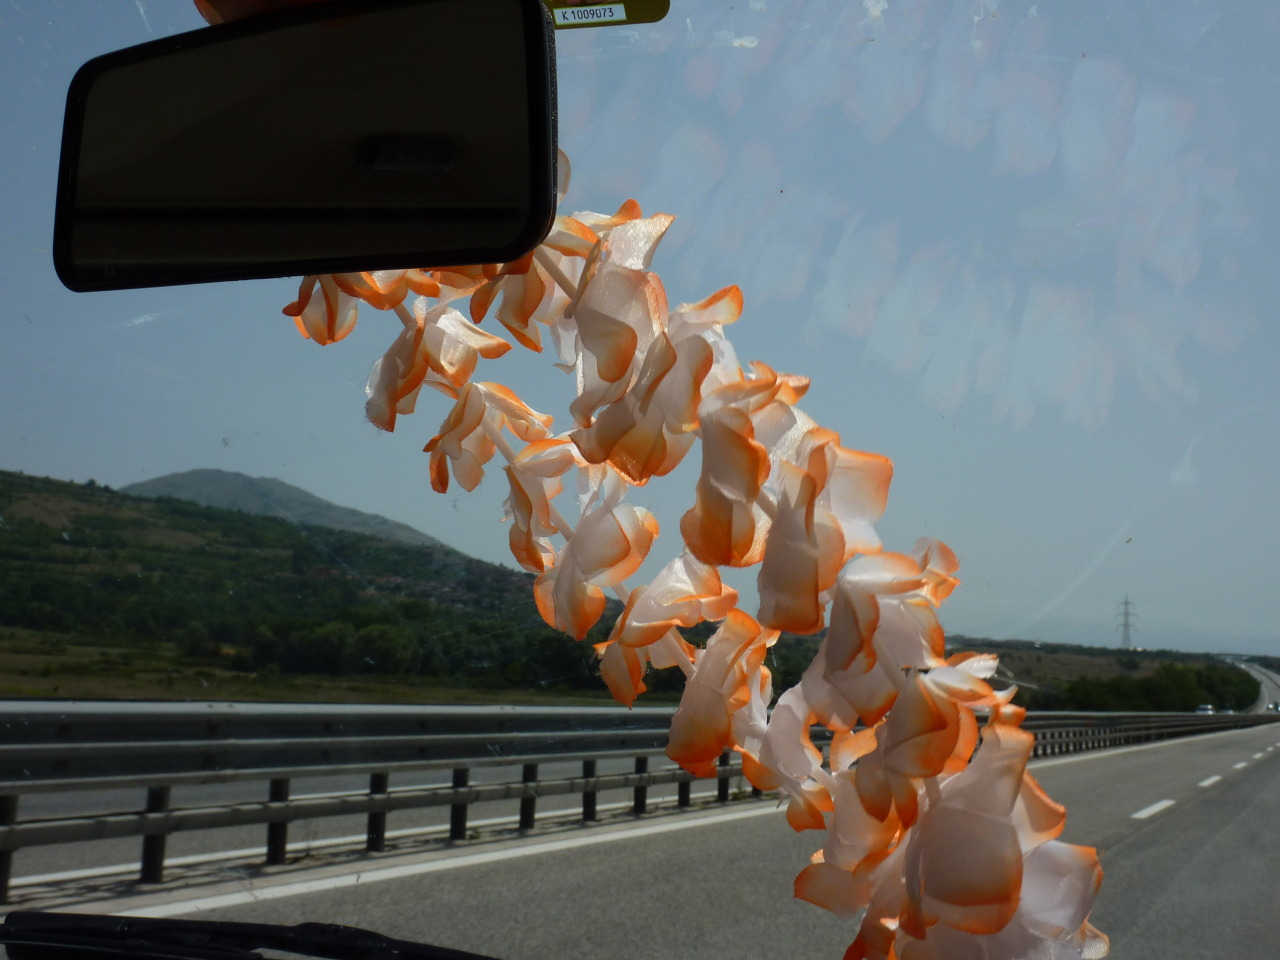
\includegraphics[width=\textwidth]{../Bilder/Sommer2012/11.jpg}
    \caption{Im Glutofen unterwegs}
    \label{img:Sommer3}
\end{figure}

\subsection{06.08.2012 Jack Sparrow alias Pepito}

\begin{wrapfigure}{R}{0.45\textwidth} 
  \begin{centering}
    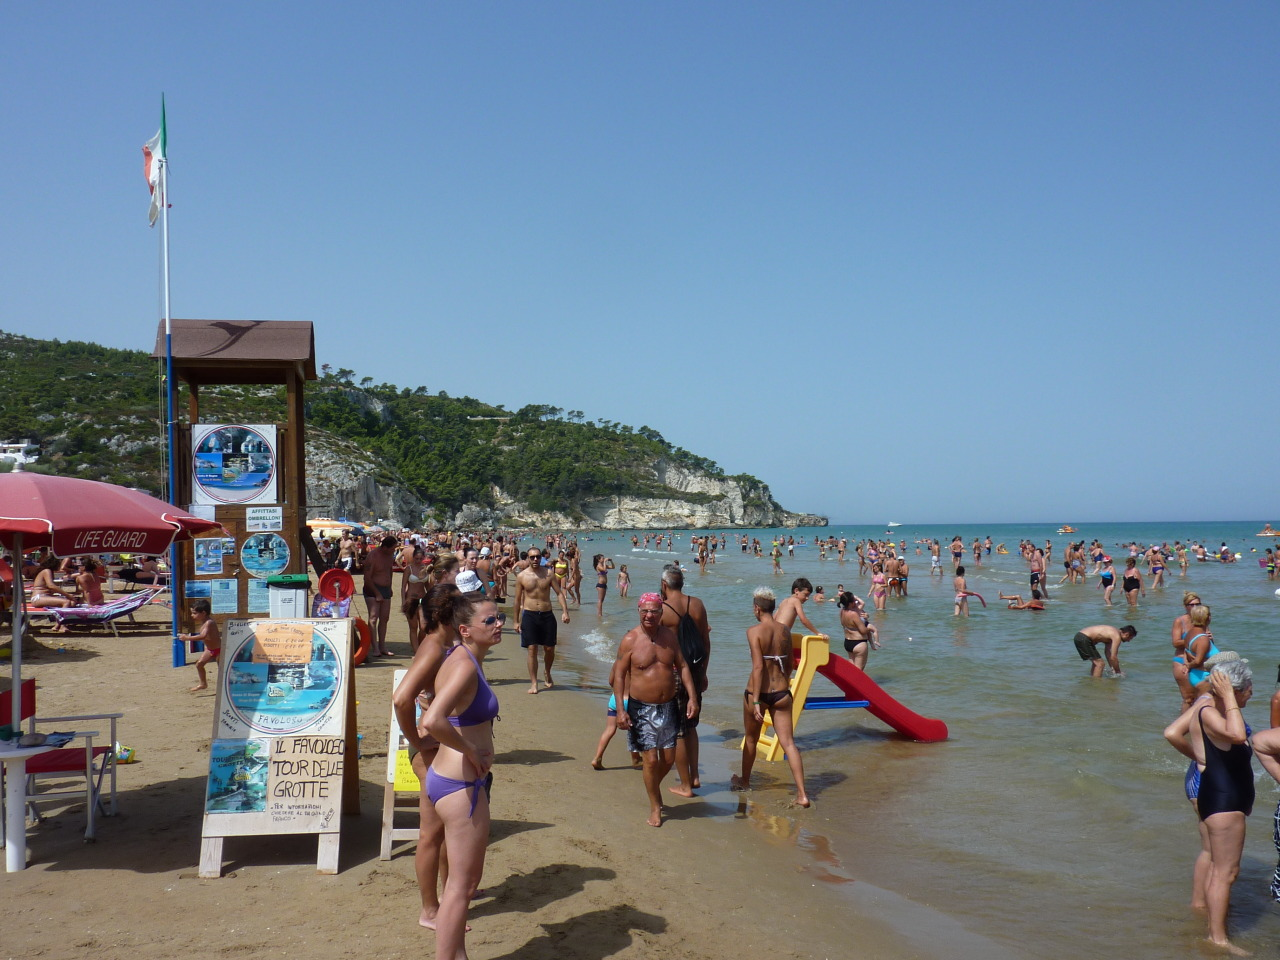
\includegraphics[width=0.4\textwidth, height=5cm, keepaspectratio]{../Bilder/Sommer2012/13.jpg}
    \caption{Action am Strand}
  \end{centering}
\end{wrapfigure} 

Die Nacht war trotz �blen Vorahnungen gar nicht so �bel.
Chantal jubelte schon fr�h am Morgen dar�ber, dass ihr hartn�ckiges Sandkorn verschwunden war.
So begann sie kurz nach 9 mit der Suche nach dem Mercato.
Wieso in aller Welt ist dieser Laden in der H�chstsaison geschlossen? Nach kurzer Absprache sattelten wir die Velos und begannen mit der Suche nach Nahrungsmittel.
Eine Tafel die mit �u�erst optimistischen 20 Meter Distanz zum Supermercato wirbt wurde rasch gefunden so wie auch der Laden der 300 Meter von der Tafel entfernt war.
Das Fr�hst�ck fiel reichhaltig aus.
Das Ameisenproblem waren wir gl�cklicherweise los.
Trotzdem machte sich jedes Brotkorn das auf den Boden fiel sofort auf den Weg Richtung Nesteingang.
Die Ameisen hier sind mindestens doppelt so gross wie in Rom und Gott sei Dank nicht an der Inneneinrichtung interessiert.
Der Weg zum Strand war kurz und schon bald waren die Liegest�hle in Beschlag genommen.
Doch was st�rte da mein sensibles Ohr? Gustavo Lima! Mindestens 50 Italiener in aller Form und Alter absolvierten eine Art Fitnesstraining am Strand.
Nach einer halben Stunde war Ruhe f�r ca.  10 Sekunden bevor der n�chste Strandabschnitt mit anderen beknackten Spielchen anfing.
Schon bald begann ich mich auf die Suche nach ein wenig Ruhe und wurde schnell f�ndig.
Ein Typ, der Jack Sparrow alt aussehen l�sst bot mir zwei Liegest�hle an, welche auch sofort besetzt wurden, nach dem ich Chantal geholt habe.
Den Rest des Tages verbrachten wir mit Faulenzen und Baden.

Am Abend stand dagegen Fitness auf dem Speiseplan... Die H�user schmiegen sich leicht erh�ht an die H�gel und genau dort wollten wir mit dem Velo hin.
Um 21 Uhr waren die Temperaturen langsam ertr�glich und wir machten uns auf den Weg, welchen wir Schweissgetr�nkt zur�cklegten.
Alle L�den hatten noch offen, dieser Umstand und die sch�nen, zahlreichen engen Gassen l�sten Gl�cksgef�hle bei Chantal aus.
Einen Teller Orechiette al Peschici f�hrten bei mir zu einer �hnlichen Reaktion.
Die Abenteuerliche Abfahrt, welche wir im Schein der Stirnlampe unter die R�der nahmen war die letzte Aktion an diesem sch�nen Tag.

\subsection{07.08.2012 Slow down..take it easy}
Heute war wieder ein Strandtag angesagt.
Doch zuerst wollten wir nochmals das sch�ne St�dtchen Peschici bei Tageslicht betrachten.
Um halb 9 Uhr machten wir uns mit dem Velo auf den Weg und hatten sogar noch Gl�ck, da der Weg weit weit hinauf teilweise im Schatten lag.
Oben angekommen streiften wir gem�tlich durch die herzigen Gassen und genossen die sch�ne Aussicht auf das t�rkisfarbene Meer.
Wir trafen sogar die Frau an, bei welcher ich gestern eine sch�ne Ledertasche geschenkt bekommen habe;) In einem Restaurant konnten wir einen feinen Kaffee geniessen, feine Croissant (eins mit Nutella;)) essen und sogar Flieger beobachten, welche im Meer Wasser f�r einen Brand hinter den H�geln holte.
Da war einer seeehr gl�cklich �ber dieses Spektakel :D Dann fetzten wir mit den Velos den Hang hinunter, gingen in den Supermercato, wo wir einen Sonnenschrim fanden, machten einen Zwischenstop im Camping und schlenderten dann zum Strand (Bei dieser Hitze kann man nicht viel schneller laufen als zu schlendern) Am Strand versuchten wir unser frisch gekauften Sonnenschirm festzumachen, was sich aber eher als schwierig herausstellte.
Der Sand war ziemlich hart.
Nach kurzer Zeit kam uns eine Italienerin zur Hilfe und zeigte uns, wie man das macht.
Endlich konnten wir uns hinlegen, sonnen, lesen, faulenzen und baden.
Heute war es sogar aushaltbar an der Sonne (f�r einige;)), da ein angenehmer Wind wehte.
Den Abend verbrachten wir mit Trinken (Bier, Campari und Wein;)) und Essen.
Hmmm ich freue mich auf die Orechiette!  

\begin{figure}[h]
   \centering
      %\subfloat[CAPTION]{BILDERCODE}\qquad
   \subfloat{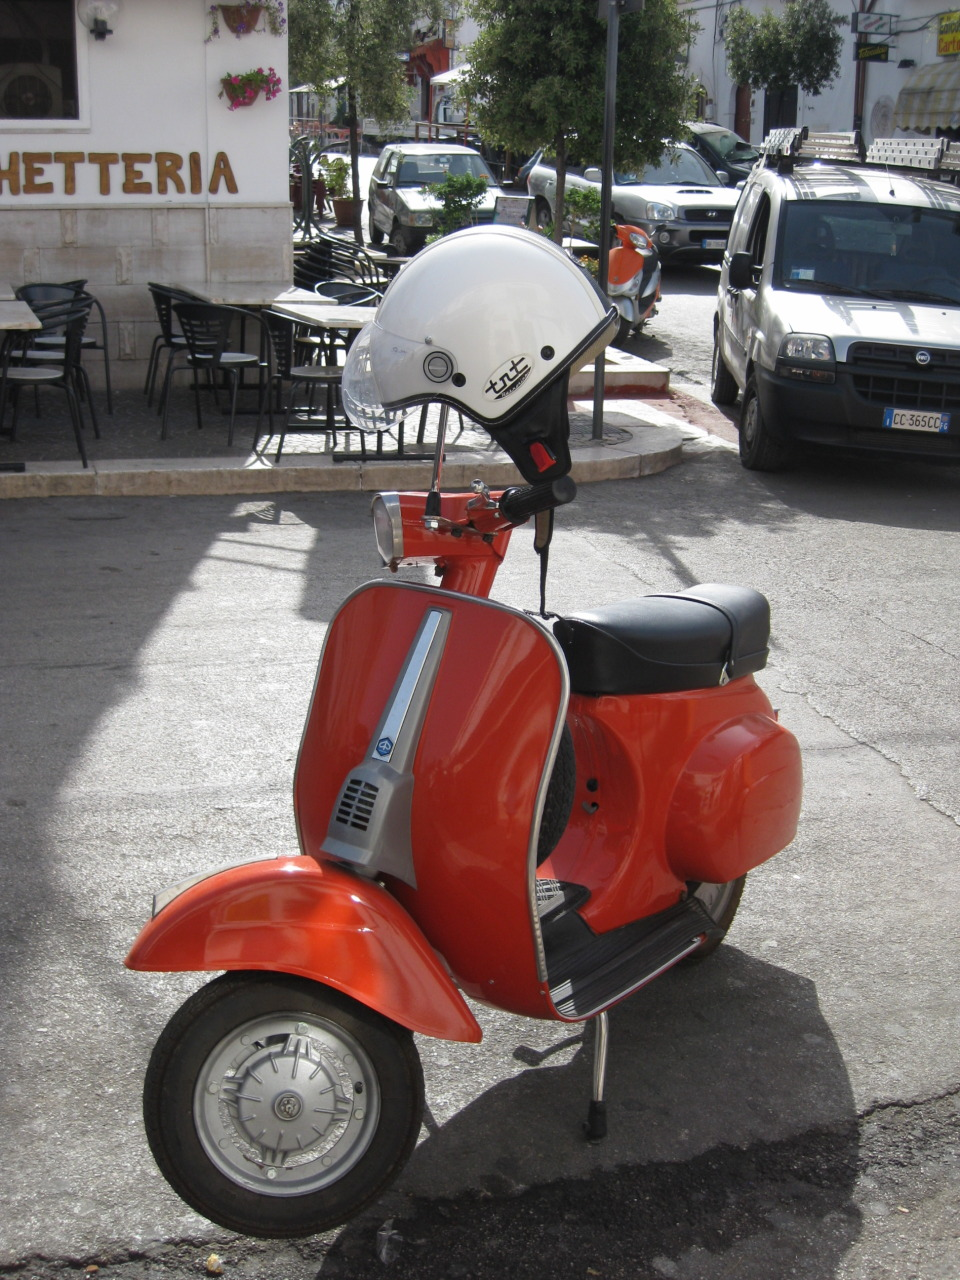
\includegraphics [width=0.3\textwidth]{../Bilder/Sommer2012/16.jpg}}\quad
   \subfloat{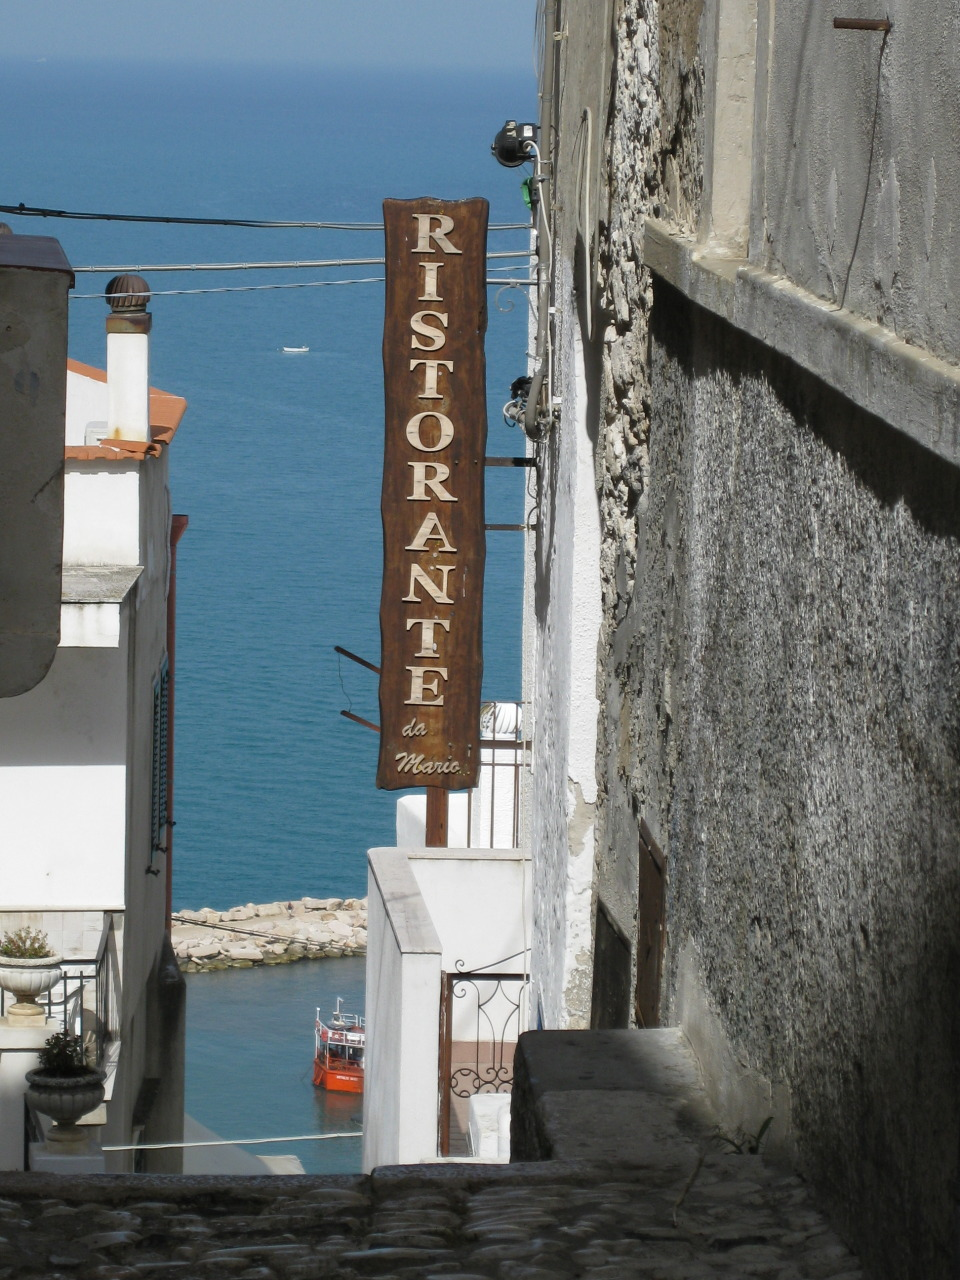
\includegraphics [width=0.3\textwidth]{../Bilder/Sommer2012/18.jpg}}\quad
   \subfloat{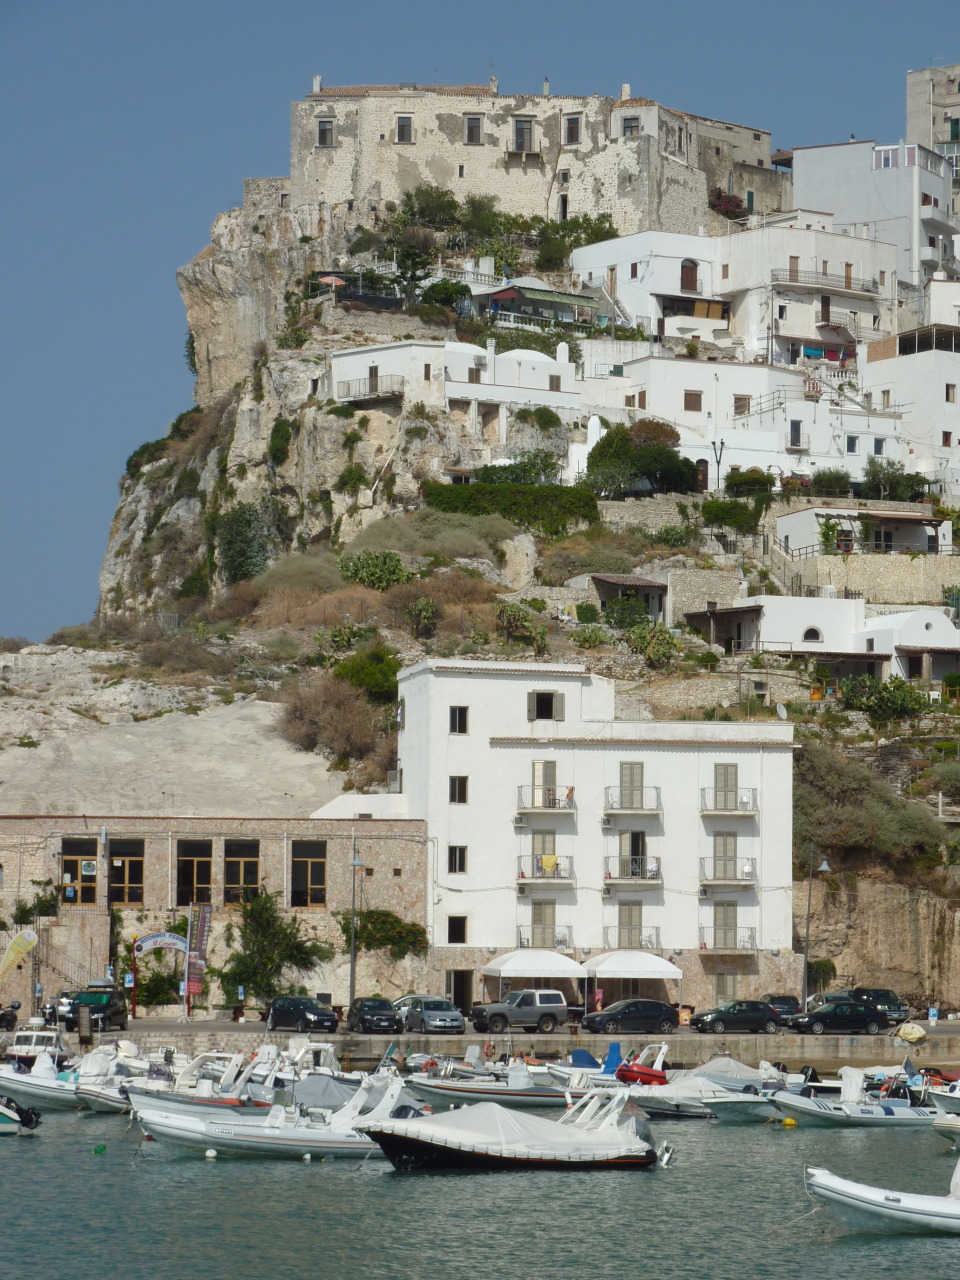
\includegraphics [width=0.3\textwidth]{../Bilder/Sommer2012/21.jpg}}\quad
   \caption[Peschici]{Peschici}
\end{figure}

\subsection{08.08.2012 Vieste}

\begin{wrapfigure}{L}{0.45\textwidth} 
  \begin{centering}
    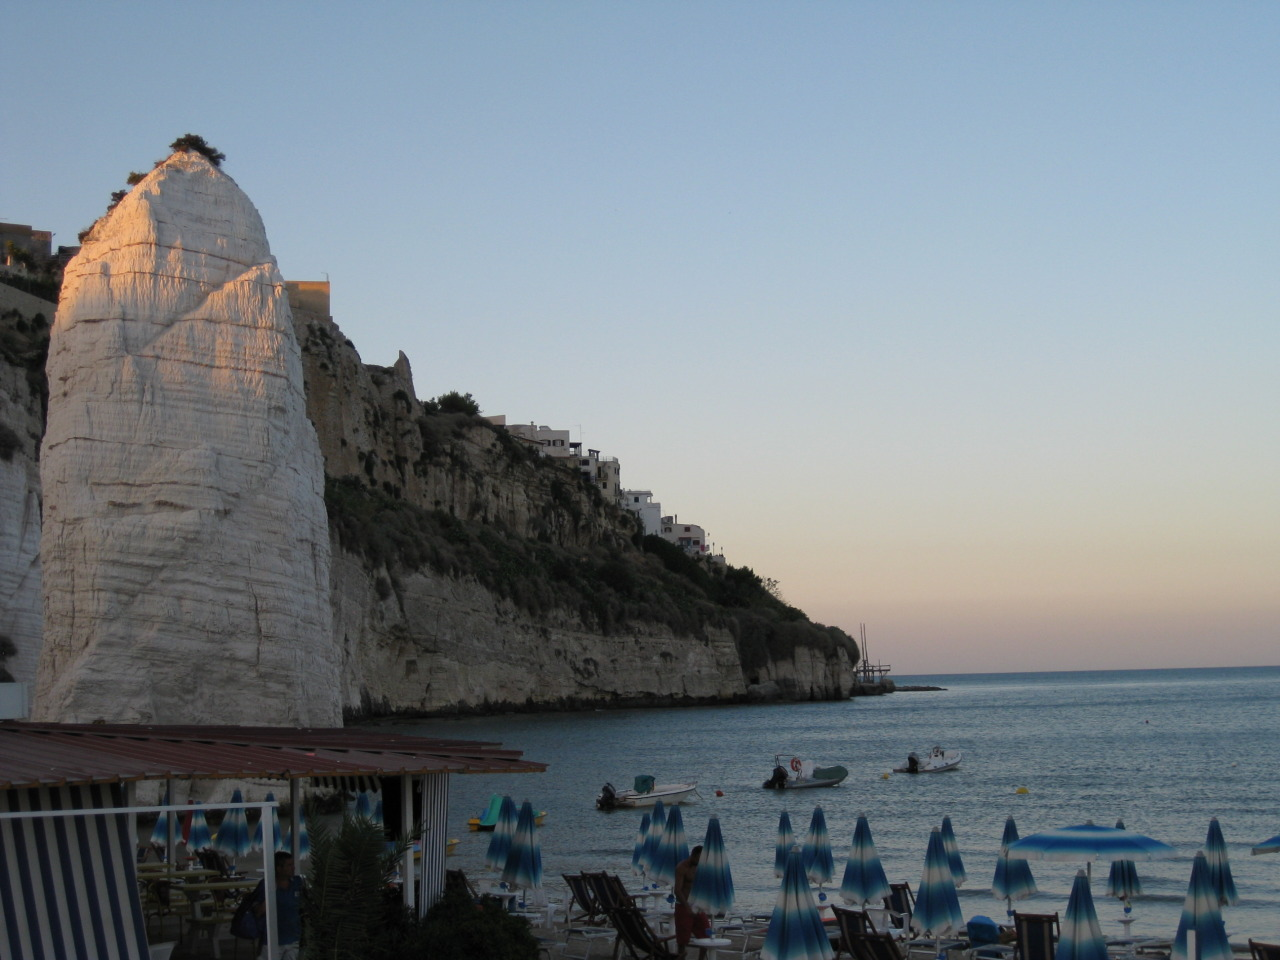
\includegraphics[width=0.4\textwidth, height=5cm, keepaspectratio]{../Bilder/Sommer2012/22.jpg}
    \caption{Vieste}
  \end{centering}
\end{wrapfigure} 

Um 12:00 mussten wir sp�testens den Campingplatz verlassen haben.
Eigentlich kein Problem, wenn da nicht die sehr aktiv anstehenden Italiener w�ren.
Nur aus Mitleid der Bedienung kam ich an die Reihe.
Normalerweise schrie bei der Frage: "`Wer ist der n�chste?"' immer eine als klassische Operns�ngerin ausgebildete Italienerin aus der dritten Reihe und bekam ihre 2 Kilogramm Mortadella vor mir.
Beim Aufr�umen fanden wir noch gewisse �berreste einer roten Fl�ssigkeit, die sich in alle Ritzen unseres Tisches eingenistet hat.
B�se Zungen behaupten es k�nnte dieselbe berauschende Fl�ssigkeit sein, welche zum umfallen des Weinglases verf�hrte (g�ll, Chantal :)) Nach dem Morgenessen waren unsere Habseligkeiten dann schnell verstaut und um 11:30 machten wir uns auf den Weg dem Meer entlang Richtung Vieste.
Das Navi war nat�rlich wieder �usserst optimistisch mit der Zeitangabe: 30 Min.
Die Fahrt war wundersch�n und schon nach einer Stunde erreichten wir Vieste und den angepeilten Campingplatz.
Dieser war sich jedoch zu Schade uns f�r 2 N�chte aufzunehmen.
Absteigende m�ssen mindestens eine Woche dort bleiben.
Nicht mit mich.
Der n�chste war dann schnell gefunden und bot zwar viel Schatten, daf�r auch sehr wenig Platz.
Egal, hauptsache sofort an den Strand, an dem ich meine zugegebenerma�en abgeschauten Sonnenschirm Eingrabtechnik stolz den nicht anwesenden Badeg�ste pr�sentierte Badeg�ste.
�ber die Mittagsstunden fl�chten diese Weicheier und Beckenrandschwimmer immer zur�ck zu ihren klimatisierten Wohnungen und Wohnw�gen.
Nur wir, sonnenverw�hnten Schweizer halten es am gl�henden Strand aus.
Der Abend n�herte sich immer mehr und meinen Versuch die Luftmatratze ohne Pumpe auf 2 Bar zu bringen scheiterten kl�glich.
An dieser umgewandelter PET Flasche befanden sich extrem effiziente Ventile.
Luft geht nicht rein und auch nicht wieder raus.
Die 3 Liter die ich in m�hsamer Arbeit in die Matratze gepresst hatte, konnte ich nun nicht wieder ablassen.

Endlich ging es Richtung Vieste.
Die ersten Schuhgesch�fte wurden durch Chantal gepl�ndert, genauso wie Attila die westliche Welt heimsuchte.
Das Restaurant direkt am Meer sorgte f�r einige Kritik (meinerseits), trotz allem war es ein sehr gelungener Abend in einer �usserst sch�nen Stadt.
Bei der Ankunft auf dem Zeltplatz durften wir noch den Kl�ngen sehr schlechter Karaokes�nger lauschen, die fehlendes Talent geschickt mit Lautst�rke zu kompensieren versuchten.
Die Sonne, die W�rme und ein wenig Campari sorgten jedoch f�r einen sehr tiefen und schnellen Schlaf trotz wildem Vibrieren von stark ge�lten Stimmb�ndern.

\begin{figure}[h]
   \centering
      %\subfloat[CAPTION]{BILDERCODE}\qquad
   \subfloat{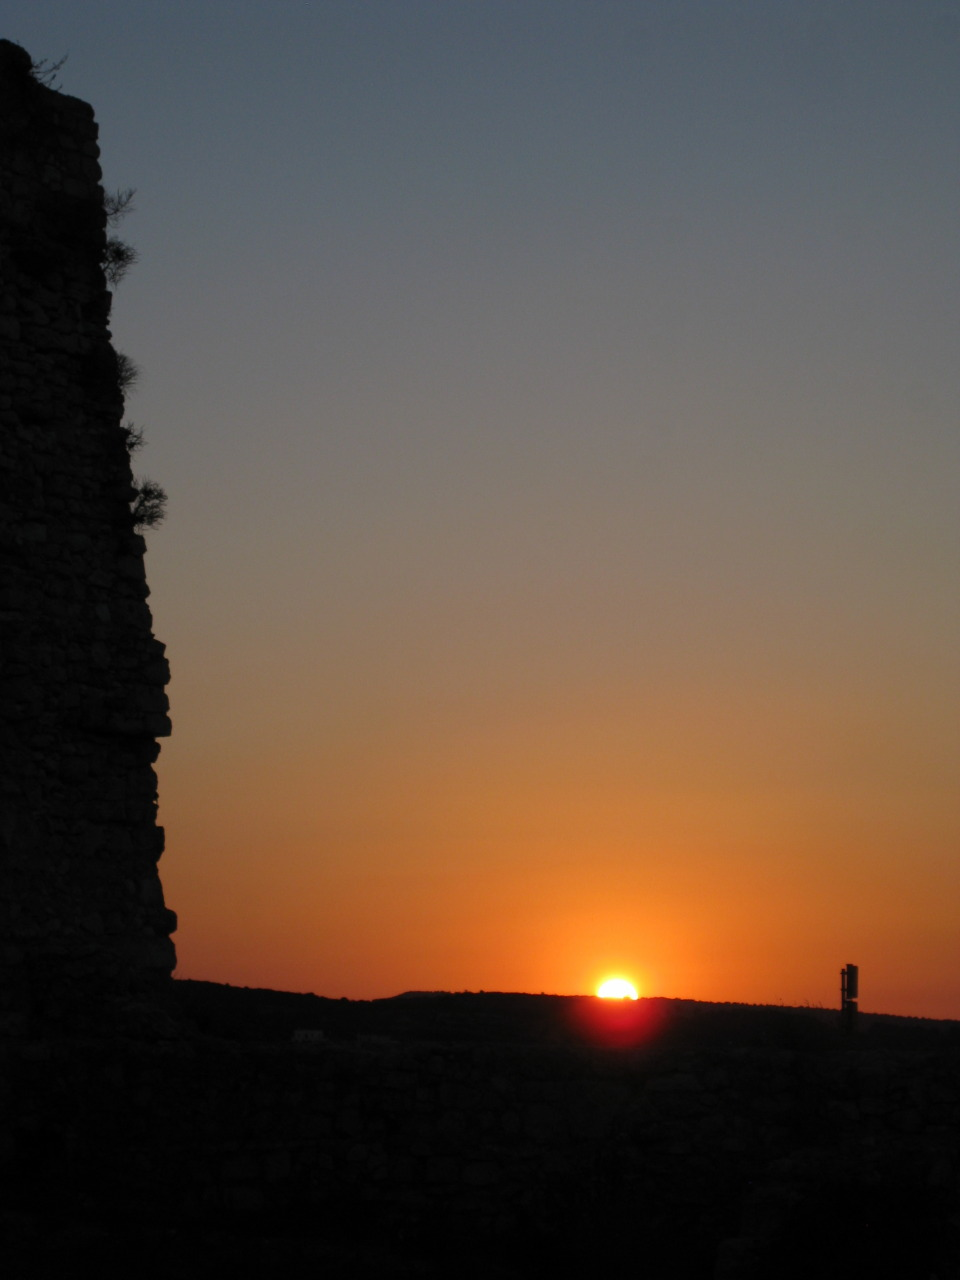
\includegraphics [width=0.3\textwidth]{../Bilder/Sommer2012/23.jpg}}\quad
   \subfloat{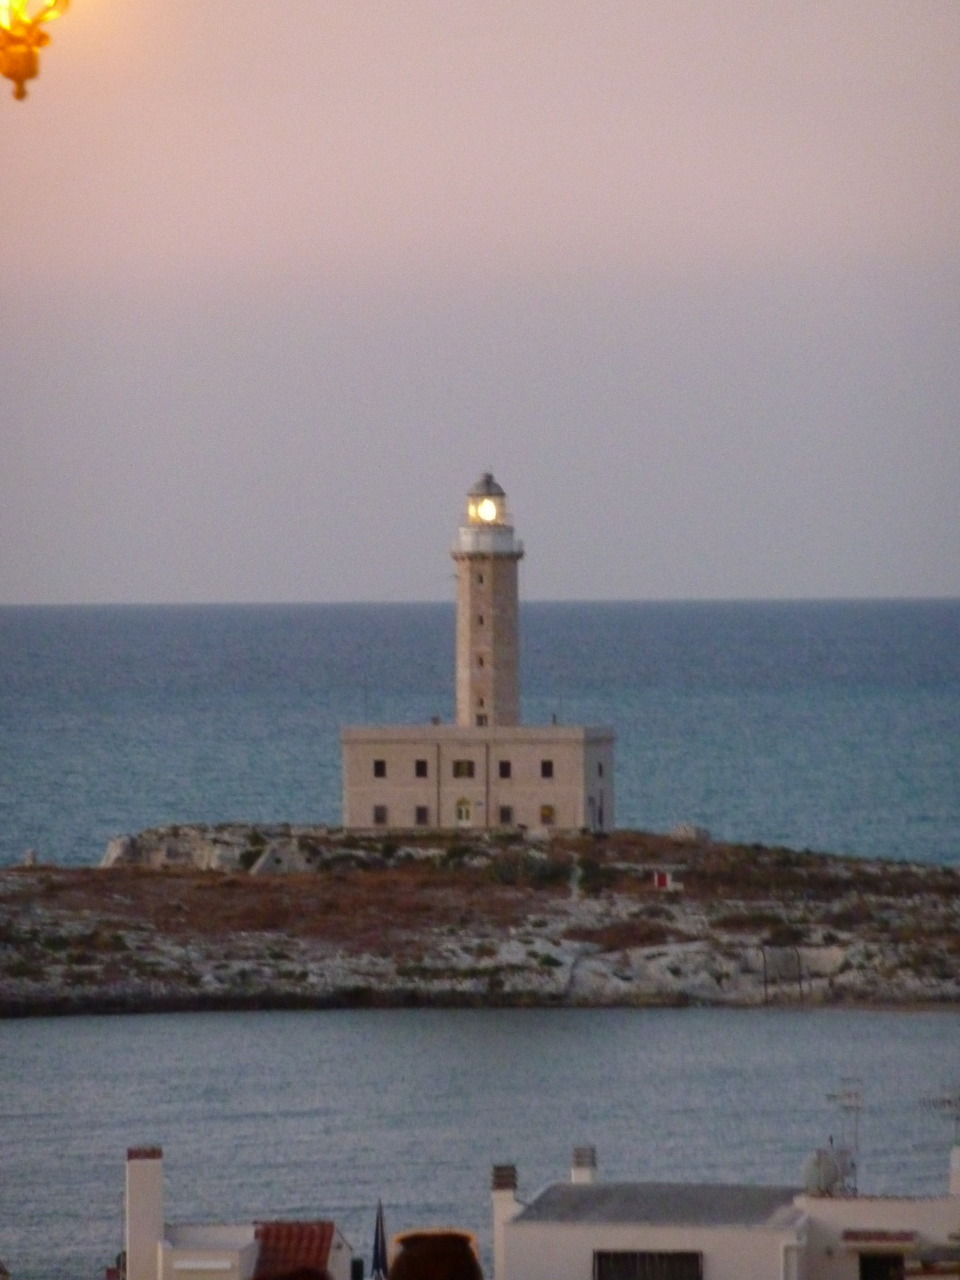
\includegraphics [width=0.3\textwidth]{../Bilder/Sommer2012/25.jpg}}\quad
   \subfloat{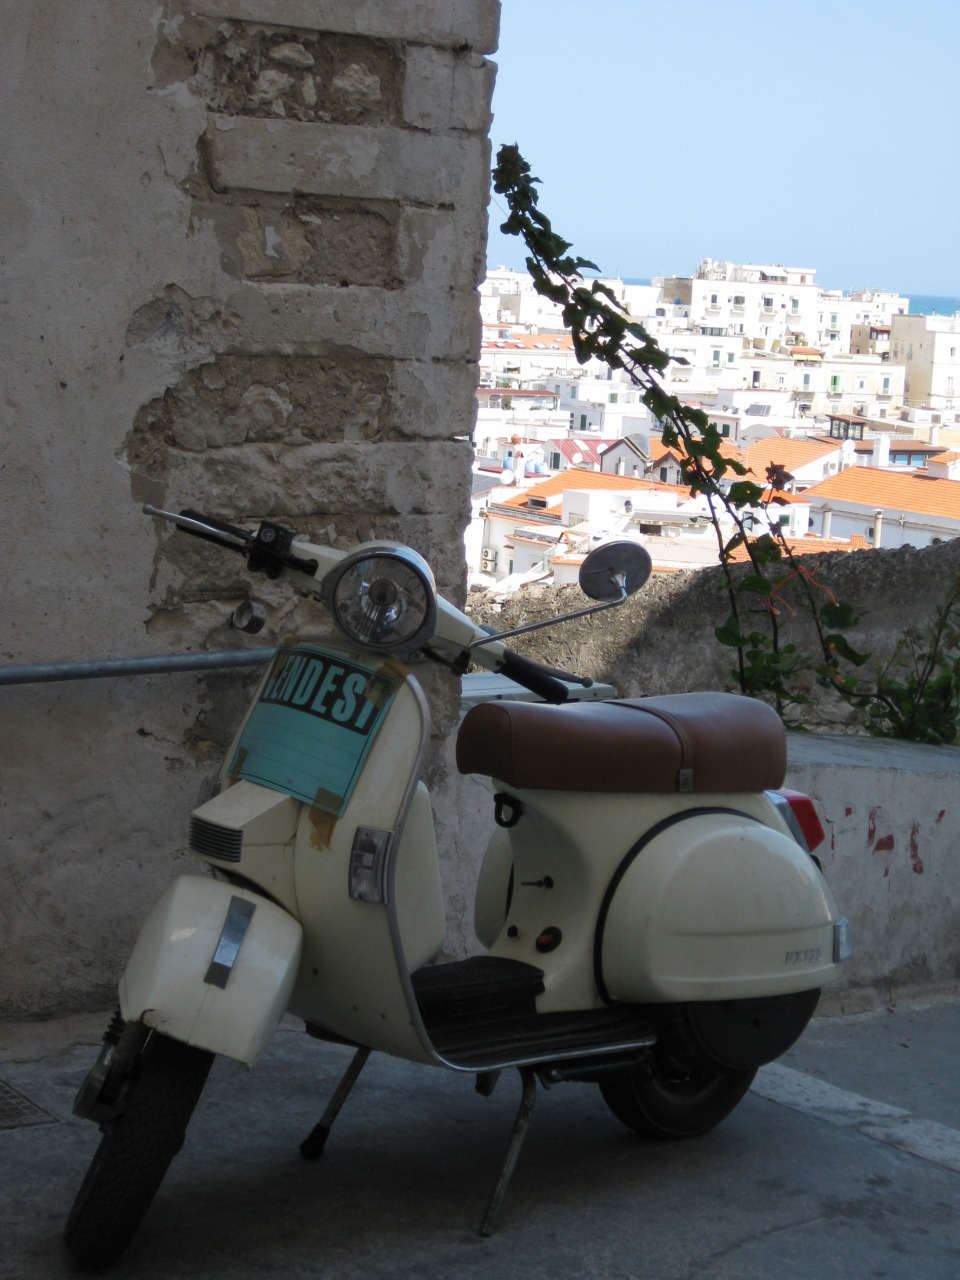
\includegraphics [width=0.3\textwidth]{../Bilder/Sommer2012/31.jpg}}\quad
   \caption[Rundgang durch Vieste]{Rundgang durch Vieste}
\end{figure}
 
\subsection{09.08.2012 Besuch der Altstadt}
Die weiteren Berichte werden sicherlich negativ beeinflusst von einem Ereignis, welches sich am 11.08.2012 ereignet hat.
Die folgenden zwei Tage waren garantiert lustiger und sch�ner als hier Beschrieben:
Ein weiteres Mal stiegen wir auf unsere Drahtesel und Radelten schon vor dem Mittag Richtung Vieste.
Dort angekommen starteten wir eine weitere Runde Sightseeing.
Viele Bilder wurden geschossen und von den n�chsten Restaurierungsobjekten getr�umt.
Den Kaffee nahmen wir bei einem Deutschsprechenden Italiener ein und genossen die Stadt bis in die Abendstunden.
Italienisch angehaucht suchten wir den Strand erst um 18:00 Uhr auf und genossen die angenehmen Abendstunden am Wasser.
Chantal konnte sich an der am Strand abgehaltenen Cha-Cha-Cha Tanzlektion kaum sattsehen.
Zur�ck auf dem nahegelegenen Camping bereiteten wir uns ein gem�tliches Abendessen vor und fielen �usserts zufrieden auf die warmen Matrazen.

\begin{figure}[H]
    \centering
    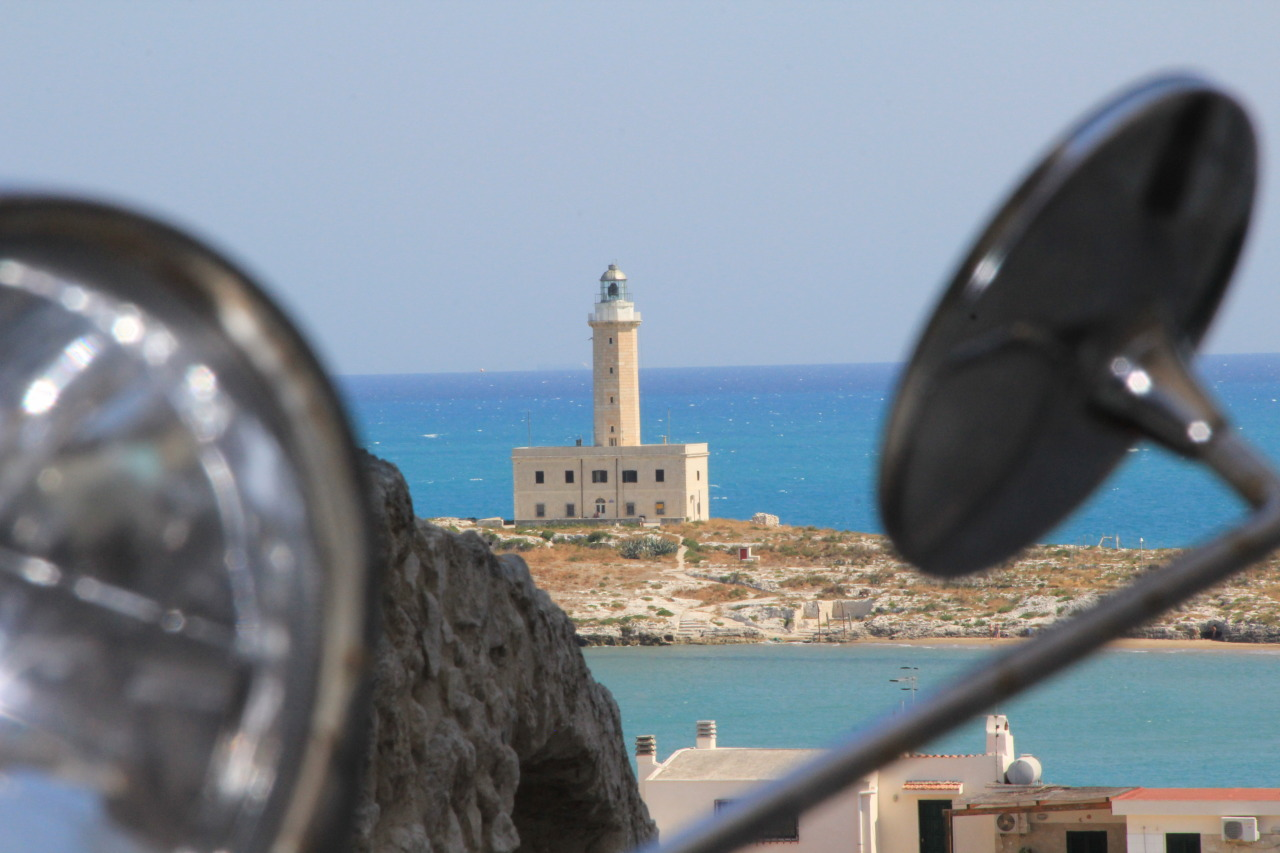
\includegraphics[width=\textwidth]{../Bilder/Sommer2012/30.jpg}
    \caption{Vespa in Vieste}
    \label{img:Sommer4}
\end{figure}

\subsection{10.08.2012 Fahrt nach Monopoli}
Auch hier mussten wir bis um 12:00 den Campingplatz verlassen haben.
Chantal besorgte das Morgenessen und ich verbrachte die Zeit mit der Vorbereitung f�r die Abfahrt.
Stolz verk�ndete ich nach getaner Arbeit eine neue Rekordzeit f�r die Aufr�umarbeiten.
Schnell gezahtl und ab ginge es auf den wundersch�n verschlungenen K�stenstra�en Richtung S�den.
Das n�chste Ziel war Trani.
Das wir mit einem kurzen Umweg erreichten.
Ein Parkplatz war schnell gefunden und die Parkanlage am Hafen wusste mehr als zu �berzeugen.

\begin{figure}[H]
   \centering
      %\subfloat[CAPTION]{BILDERCODE}\qquad
   \subfloat{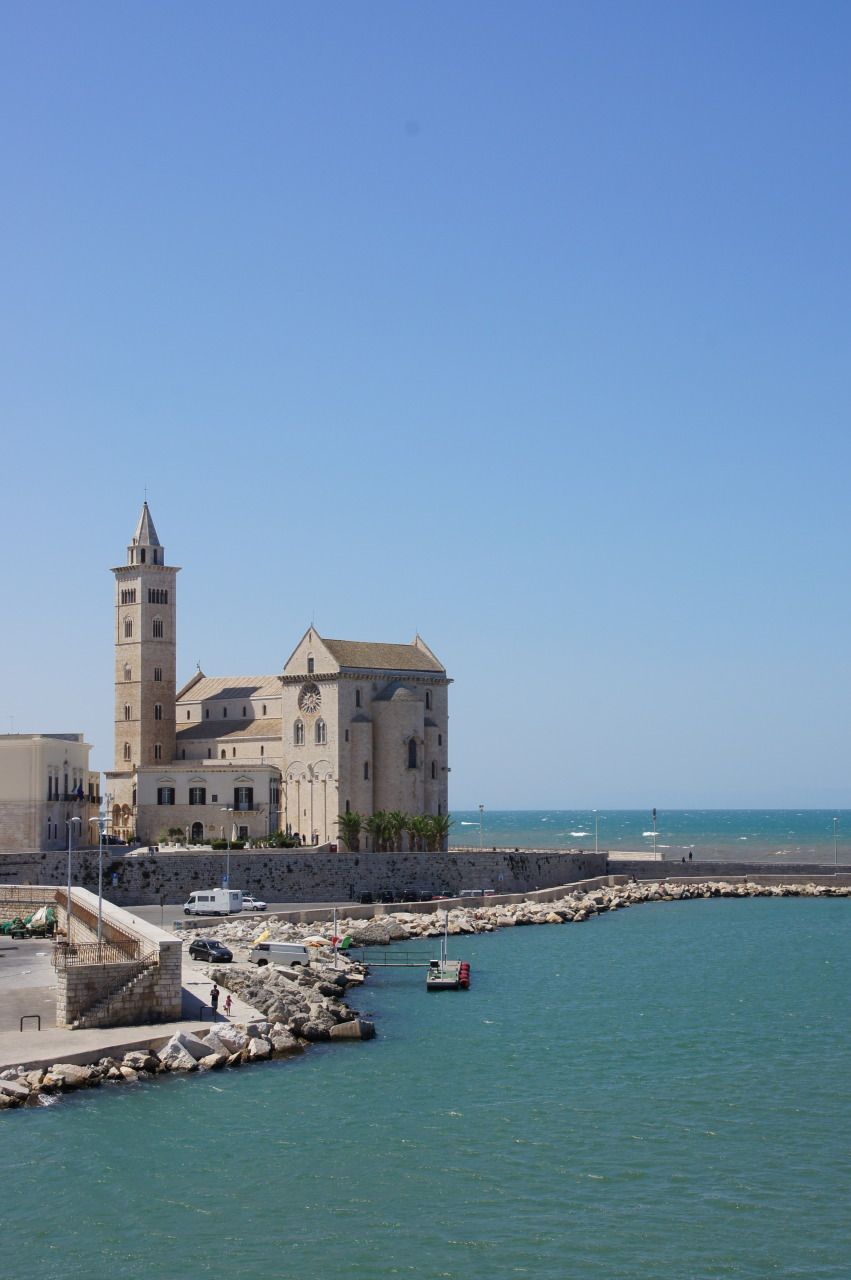
\includegraphics [width=0.3\textwidth]{../Bilder/Sommer2012/38.jpg}}\quad
   \subfloat{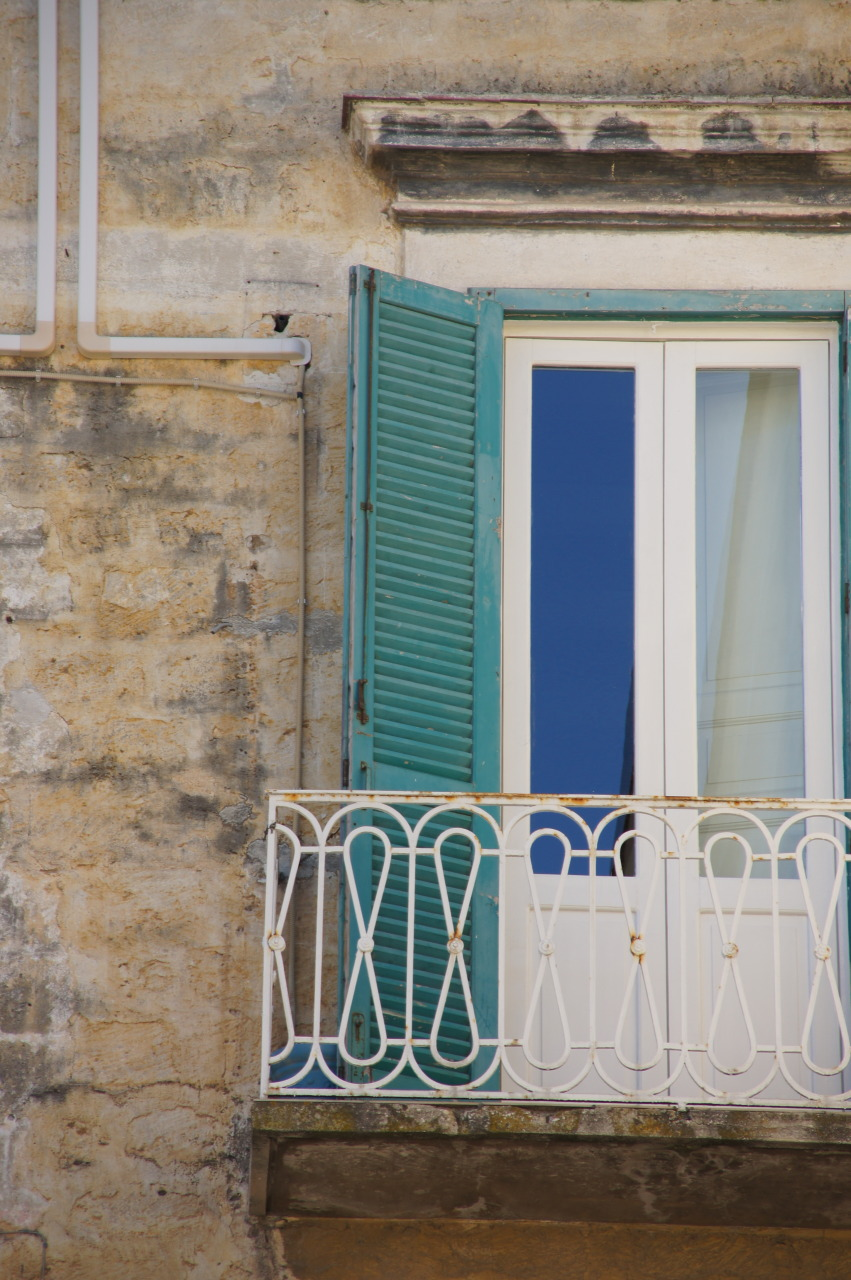
\includegraphics [width=0.3\textwidth]{../Bilder/Sommer2012/40.jpg}}\quad
   \subfloat{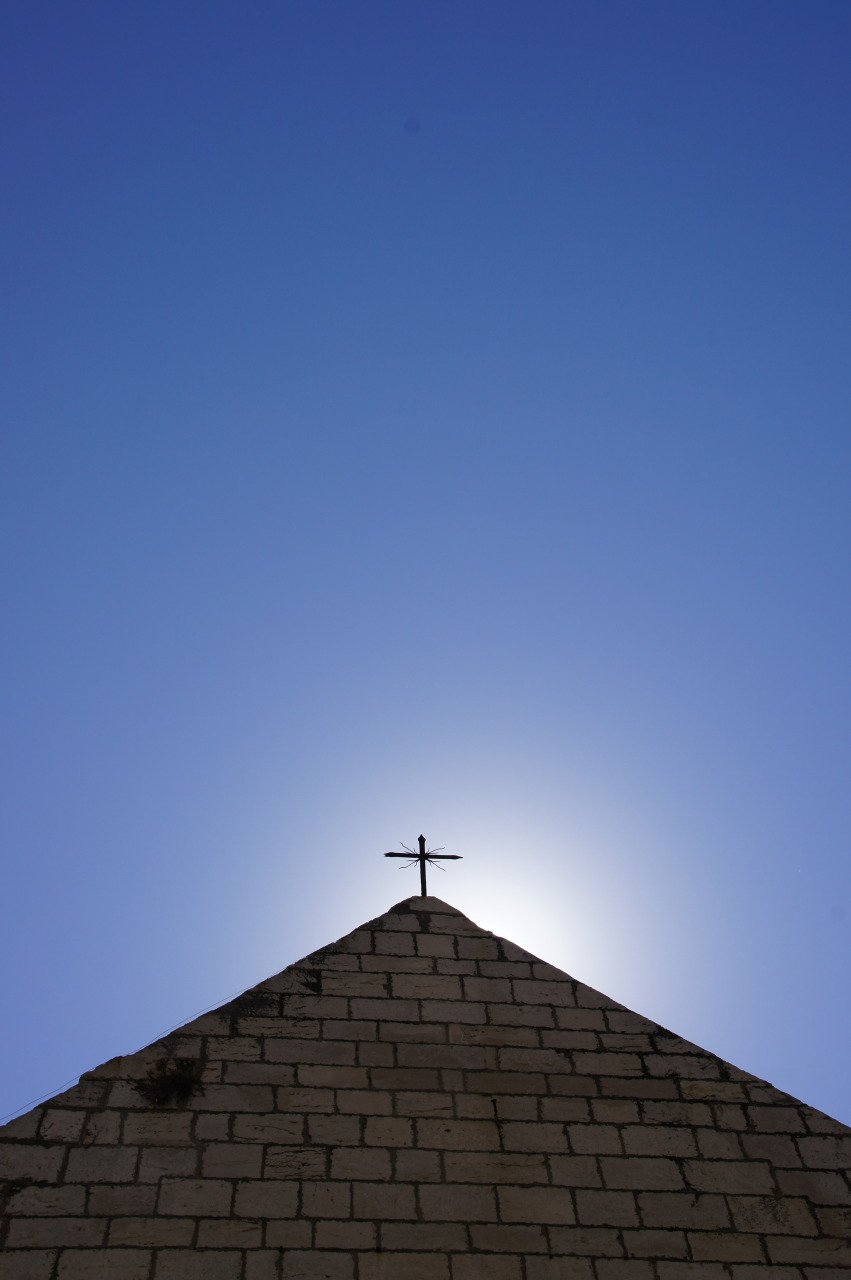
\includegraphics [width=0.3\textwidth]{../Bilder/Sommer2012/41.jpg}}\quad
   \caption[Trani]{Trani}
\end{figure}

Ganz im Gegenteil zur Altstadt.
Als Entschuldigung muss hier aufgef�hrt werden dass zwar Siesta war, trotzdem glich das ganze einer Geisterstadt.
Einzelne Touristen schlurften durch die Gassen, alles andere war leer.
Eine Bar, welche ge�ffnet hat war nicht auszumachen.
Schlussendlich nahm uns ein Restaurant auf, bei dem sich die Bedienung �ber unsere sehr begrenzte Bestellung wunderte.

\begin{figure}[H]
    \centering
    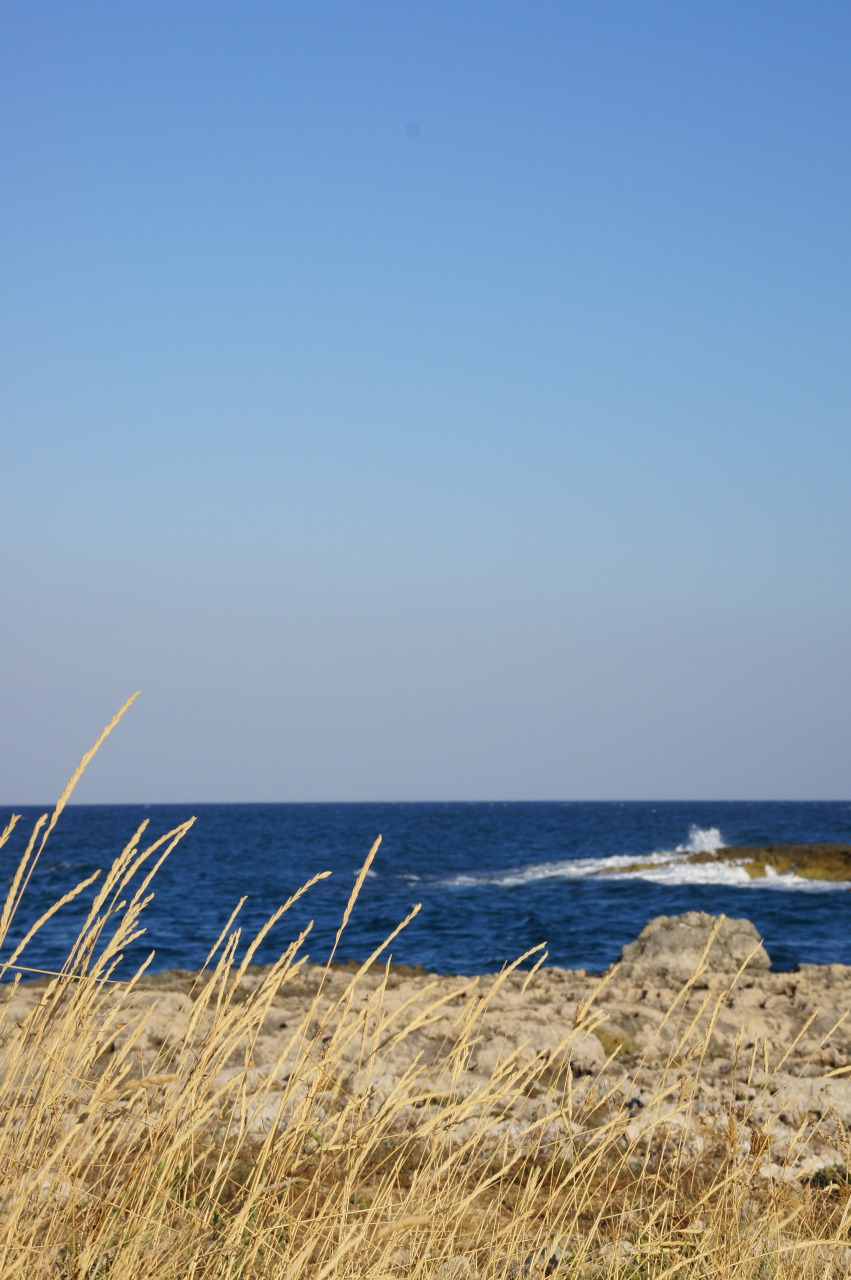
\includegraphics[width=0.5\textwidth]{../Bilder/Sommer2012/43.jpg}
    \caption{An der K�ste bei Monopoli}
    \label{img:Sommer4}
\end{figure}

Nach dem der Bus wiedergefunden war, ging es weiter auf der SS 16 Richtung Bari/Brindisi.
Der Verkehr um Bari verhie� nichts positives f�r die baldige Wiederkehr am n�chsten Dienstag.
Der Reisef�hrer versprach schon keine Anh�ufung von Campingpl�tzen mehr und tats�chlich machten sich die begehrten Abstellpl�tze �u�erst rar.
Bei einem ersten kurzen Besuch von Polignano al Mare konnten wir keinen Campingplatz ausfindig machen.
4 km s�dlich von Monopoli hatten wir dann mehr Gl�ck.
San Stefano nahm uns in Empfang.
Die Einweisung auf den Platz nahm ein �bereifriger Ciao fahrender Platzgehilfe vor.
Wie wurden in Mitten von Dauercamper platziert.
Als ich den Versuch unternahm Jack auf dem Platz zu wenden, kam er mit lautem Zweitaktgeknatter angebraust und wies uns wild fuchtelnd vermutlich auf irgendetwas hin.
Wir verstanden nur das wir den Bus wieder drehen mussten.
Jedoch reichte so unsere Kabelrolle nicht bis zur n�chsten Elektrizit�t spendenden Pfosten.
Genau in diesem Augenblick durchzog es mich wie vom Blitz getroffen.
Ich hatte in Vieste den Adapter auf die lustigen Euro Stecker stecken gelassen.
SHIT, so viel zu der Bestzeit im Aufr�umen.
Ohne Strom kein K�hlschrank, kein
... und so weiter.
Ich h�tte mich schlagen k�nnen.
Der Besuch am Camping eigenen Strand bes�nftigte die Gem�ter wieder.
Pl�ne f�r eine Neubeschaffung wurden gemacht und Routen f�r das Velo nach Monopoli verglichen.
Ab ging es.

Die Stadt war wundersch�n von einer hellen Stadtmauer einges�umt.
Schmuckgesch�fte lockten und schon bald trafen wir auf dem Hauptplatz ein um einen gem�tlichen Ap�ro zu geniessen.
Noch schnell eine Flasche Wein gekauft und zur�ck ging es mit der Suche nach unseren Fahrr�dern.
Die Fahrt verlief durch absolute Dunkelheit und nur unsere Stirnlampen und das Velolicht verhalfen uns zu einer eingeschr�nkten Sicht auf die Strasse.
Auf dem Campingplatz angekommen wehte uns ein starker Wind entgegen.
Keine Chance auf ein gem�tliches Kochen vor dem Bus.
Also die "`K�che"' im Bus montiert und nach kurzer Zeit wurde das Abendessen serviert.
Noch kurz einen Film auf dem Laptop angeschaut und dann friedlich wurde friedlich einged�st.

P.S. Der Wein blieb an diesem Abend unangetastet. Ger�chten zu Folge war der Ap�ro daran Schuld.

\subsection{11.08.2012 Wundersch�ner Tag der am Abend leider eine sehr negative Wendung nahm.}
Das ist er also nun, unser Schicksalstag. 
Aber zuerst vorne Angefangen: Nach dem Morgenessen und dem Aufsuchen des Mercato (Eher eine Bar als ein Mercato... anyway) begaben wir uns ans Meer.
Leider war der Aufenthalt dort zeitlich begrenzt, da die augenscheinlich strenge Campingleitung mit Ciao-betriebenen Hilfssheriff, eine Fahrverbotszeitzone eingerichtet hat.
Ab 13:30 bis 16:00 war jeglicher Verkehr untersagt.
Jack machte schon bei den wilden Rangierversuchen mit seinem lockeren Auspuff auf sich aufmerksam und so versuchten wir wenn immer irgendwie m�glich uns an die Spielregeln zu halten.
Am Strand war der Kindergarten los.
Chantal am�sierte sich k�niglich �ber das wilde Treiben.
Andere verlie�en fluchtartig den Tatort.

\begin{wrapfigure}{L}{0.45\textwidth} 
  \begin{centering}
    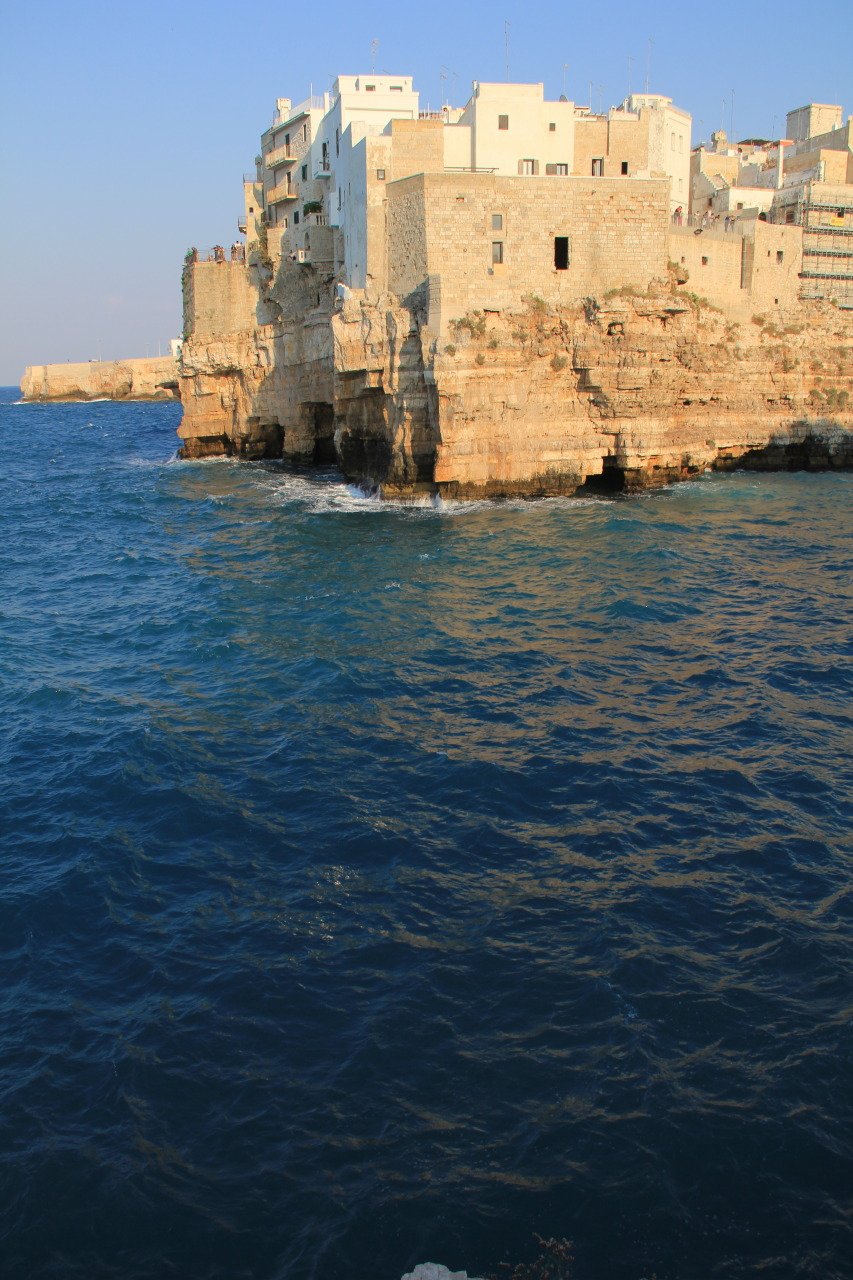
\includegraphics[width=0.4\textwidth, height=5cm, keepaspectratio]{../Bilder/Sommer2012/54.jpg}
    \caption{Polignano al Mare}
  \end{centering}
\end{wrapfigure} 

Kurz nach 13:00 Uhr machten wir uns auf den Weg mit Sack und Pack um Polignano einen Besuch abzustatten.
Der Reisef�hrer versprach einen Parkplatz im Norden der Stadt und nach einem kurzen Besuch an der Tankstelle befanden wir uns dort, jedoch der Parklpatz war nicht in Sicht.
Ein Feld bot sich jedoch als L�sung f�r das leidige Problem an.
Auf diesem waren auch schon mehrere Autos parkiert.
Beim Eingang mehrere langatmige Italienische Schilder.
Jack wurde platziert und die Stadt mit meinem Fotoapparat erobert.
Das eigentliche Ziel war ein Restaurant, welches wir am Abend besuchen wllten.
Dazwischen nutzten wir die Zeit f�r Sightsseing, Suche um wieder Pfus f�r den Bus zu bekommen und Ap�ros.
Mein Handy entschied sich nicht mehr zu funktionieren und eine kurze R�ckfrage mit Nordeuroa ergab des Swisscom aussnahmsweise nicht Schuld daran sein sollte.
Viele Fotos sp�ter traffen wir kurz nach 20:00 Uhr zum Essen ein und bemerkten, dass uns der Campingplatz nur bis 22:30 zur�ck auf den Platz lassen w�rde.
Der Zweiakt-Cowboy w�rde uns sonst den Zutritt verweigern.
Ziemlich genau um 22:00 waren wir nach einem genialen Men� zur�ck beim Bus und machten uns sofort auf den Weg Richtung Monopoly.

Der Deputy erwartete uns schon an der Eingangspforte und wies mittels wilden Handzeichen daraufhin Ruhe zu bewahren.
Dass sollte er erstmals versuchen Jack beizubringen... Chantal verschwand direkt auf dem Stillen �rtchen.
Beim zur�ck r�umen des Gep�cks wurde mir ziemlich schnell klar das gewisse Sachen fehlen.
Ein kurzer Blick auf das Schloss der Seitent�re best�tigte leider den Verdacht das Jemand den Schl�ssel mit dem meist orangenen Griff und der Gr�sse 4 verwendet hat.
KAAACCKKKEEE.
Mein Rucksack, der Rucksack von Chantal, die Kameratasche von Chantal nat�rlich mit Inhalt, die neue Ledertasche und beide Necessaires hatten einen neuen unrechtsm�ssigen Besitzer gefunden.
Leider ein sehr unsch�ner Ausklang eines sonst sch�nen Tages.

\begin{figure}[H]
   \centering
      %\subfloat[CAPTION]{BILDERCODE}\qquad
   \subfloat{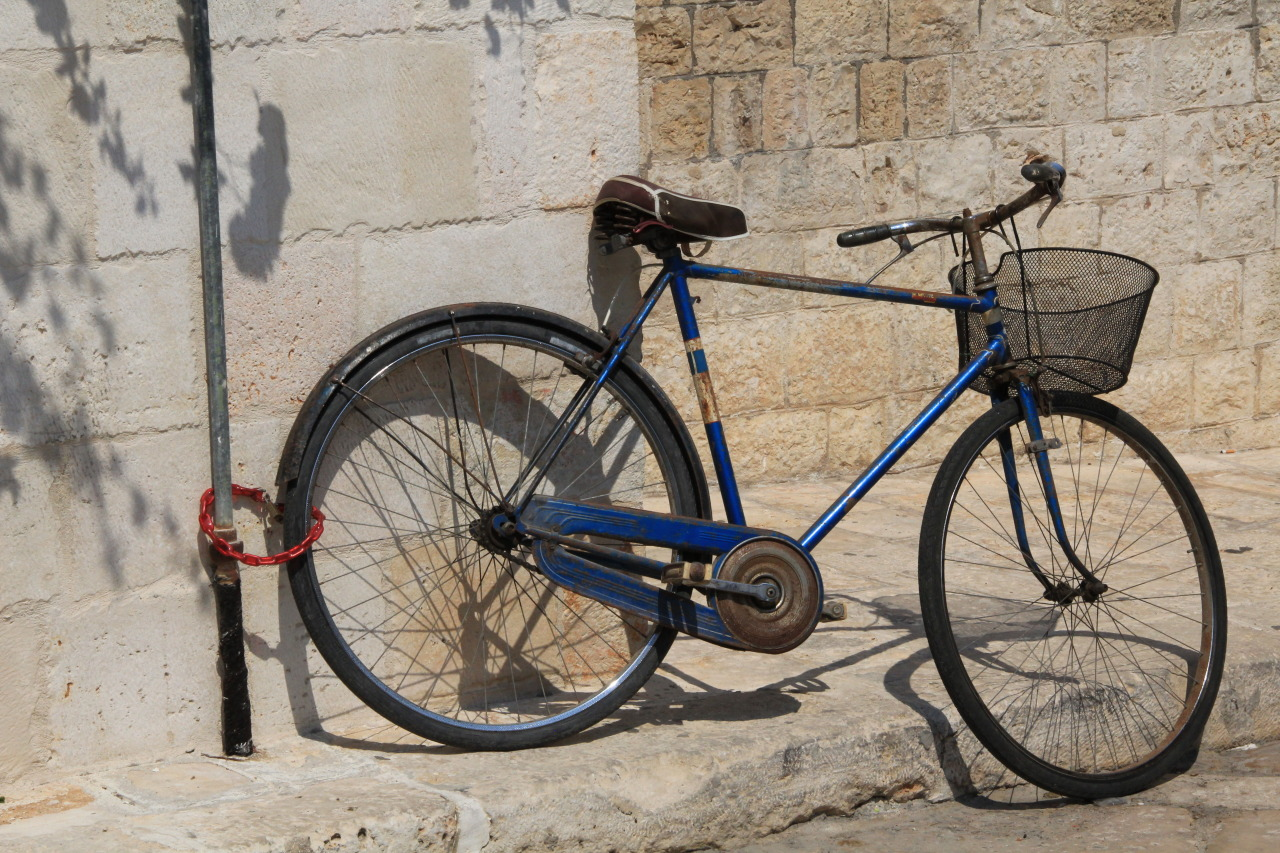
\includegraphics [width=0.3\textwidth]{../Bilder/Sommer2012/50.jpg}}\quad
   \subfloat{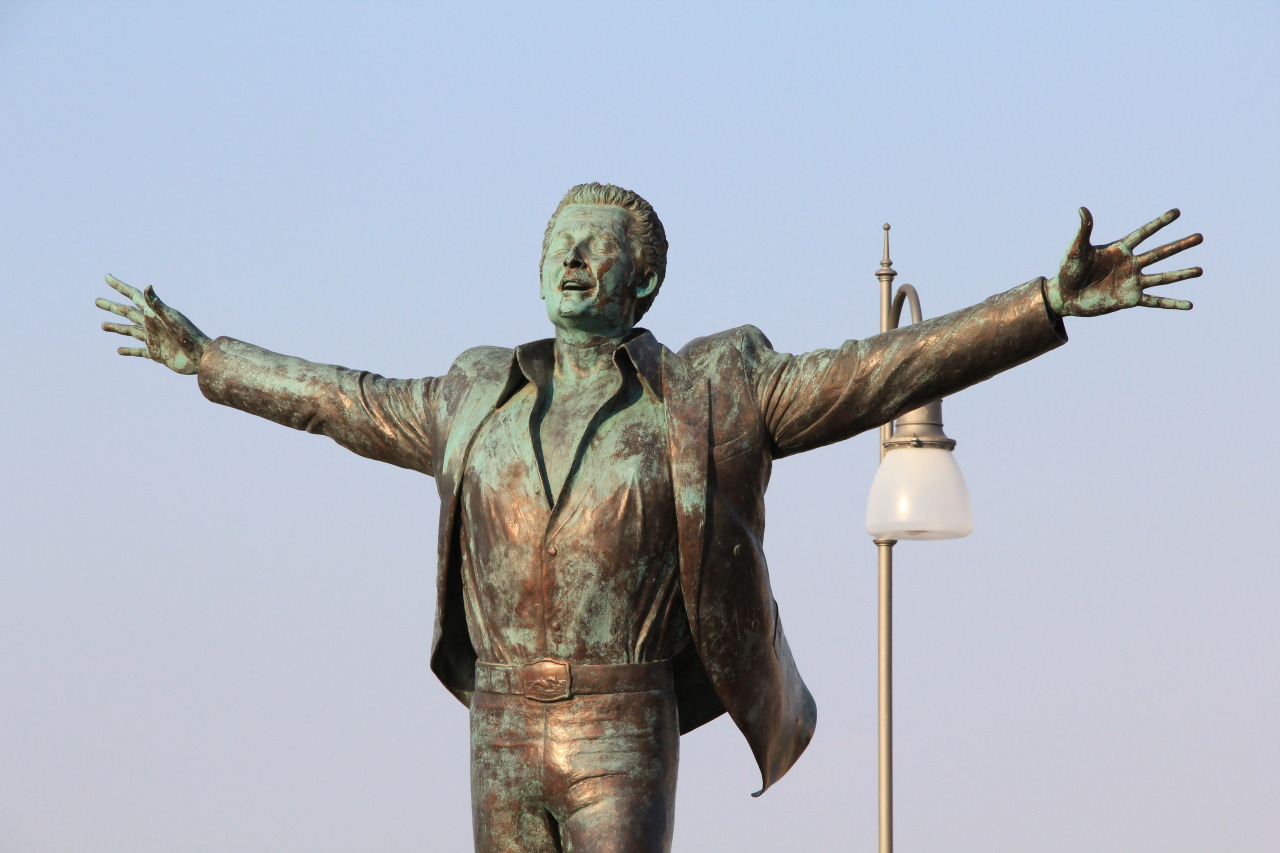
\includegraphics [width=0.3\textwidth]{../Bilder/Sommer2012/52.jpg}}\quad
   \subfloat{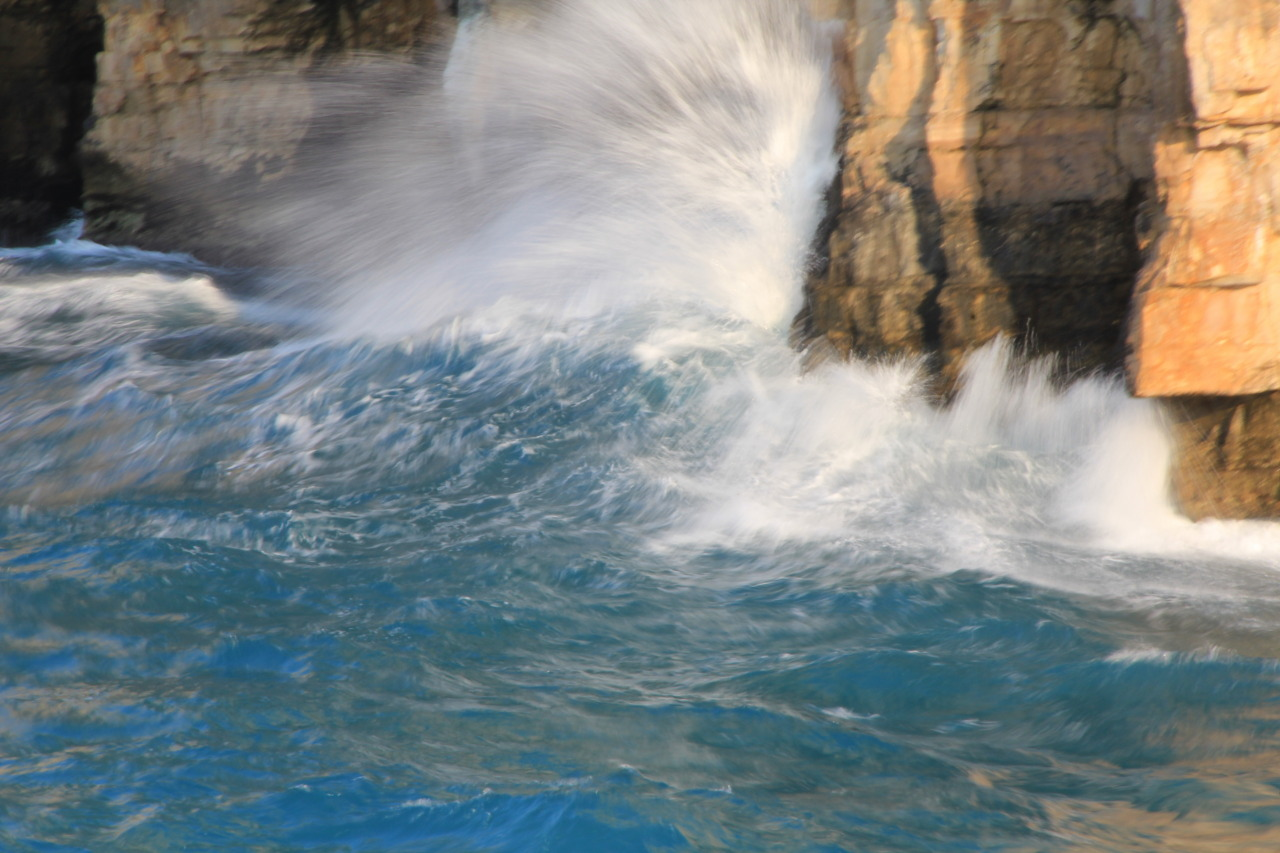
\includegraphics [width=0.3\textwidth]{../Bilder/Sommer2012/53.jpg}}\quad
   \caption[Polignano al Mare]{Polignano al Mare}
\end{figure}

\subsection{12.08.2012 Warten auf die Polizei}

\begin{wrapfigure}{L}{0.45\textwidth} 
  \begin{centering}
    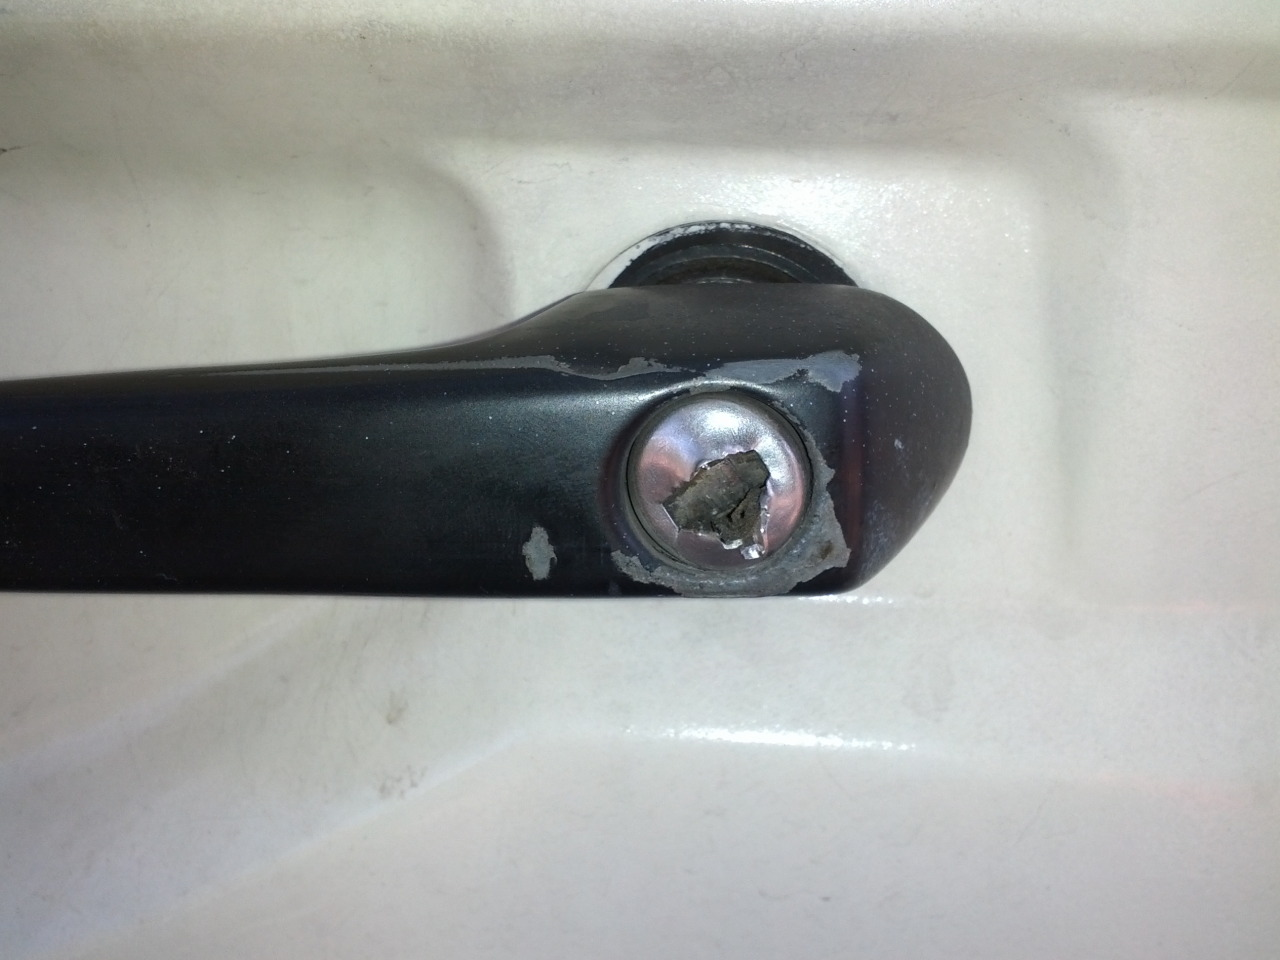
\includegraphics[width=0.4\textwidth, height=5cm, keepaspectratio]{../Bilder/Sommer2012/59.jpg}
    \caption{Ehemaliges Schloss}
  \end{centering}
\end{wrapfigure} 

Wir wollten den Diebstahl nat�rlich m�glichst schnell der Polizei mitteilten und wenn m�glich noch einmal einen kurzen Blick an den Tatort werfen.
Kurz vor 11 Uhr nach dem wir uns neue Zahnb�rstchen und Zahnpaste organisiert hatten ginge es zur�ck nach Polignano.
Zuerst jedoch wurden wir von den H�tern des Campingplatzes, welche ihr kleines Reich verteidigen m�chten, zur�ckgepfiffen.
Bei der Entsorgung des Abfalls hatten wir anscheinend einen Fehler begangen, der jedoch auch mittels Italienischen Fluchtiraden nicht behoben werden konnte.
Die Suche beim Parkplatz ergab leider kein nennenswertes Resultat.
Der \glqq Parkplatz\grqq war auch heute wieder gut besucht, trotzdem wollten wir uns m�glichst schnell aus dem Staub machen, da auch der Ersatzschl�ssel von Chantal im geklauten Gep�ck war.
Dank der Suche nach dem Adapter f�r die Stromversorgung wussten wir schon wo sich das Polizeirevier befand und steuerten nach dem mehrmals kontrollierten Abschlie�en des Busses genau dieses an.
Der kahlk�pfige Beamte wies uns sofort an das Touristenb�ro aufzusuchen, da er nur italienisch sprach.
Die sich M�he gebende Angestellte des Touri-B�ros verwies und nach kurzer R�cksprache mit dem Polizisten eine T�re weiter an die Carabinieri
Nach 10 min Suchen fanden wir auch diese Geb�ude und darin ein mit Orden behangener Ordnungsh�ter.
Wir hofften schon das die H�lfte der glitzernden Plaketten f�r ausserodentliche Englischkenntnisse verliehen wurde, wurden aber leider arg ent�uscht, Der gute Mann versuchte sich geschickt mit Ausreden in die nahende Siesta zu fl�chten und stellte sich dumm und taub.
Mit etwas Geduld fanden wir heraus, dass ein Kollege (des Englisch m�chtig) um 16:00 Uhr an selber Stelle anwesend sein sollte.
Die Zeit dazwischen lagen wir am viel besuchten und noch mehr fotografierten Strand von Polignano und deckten uns mit den Artikel ein, die vom Saupack geklaut worden sind.

\begin{figure}[H]
   \centering
      %\subfloat[CAPTION]{BILDERCODE}\qquad
   \subfloat{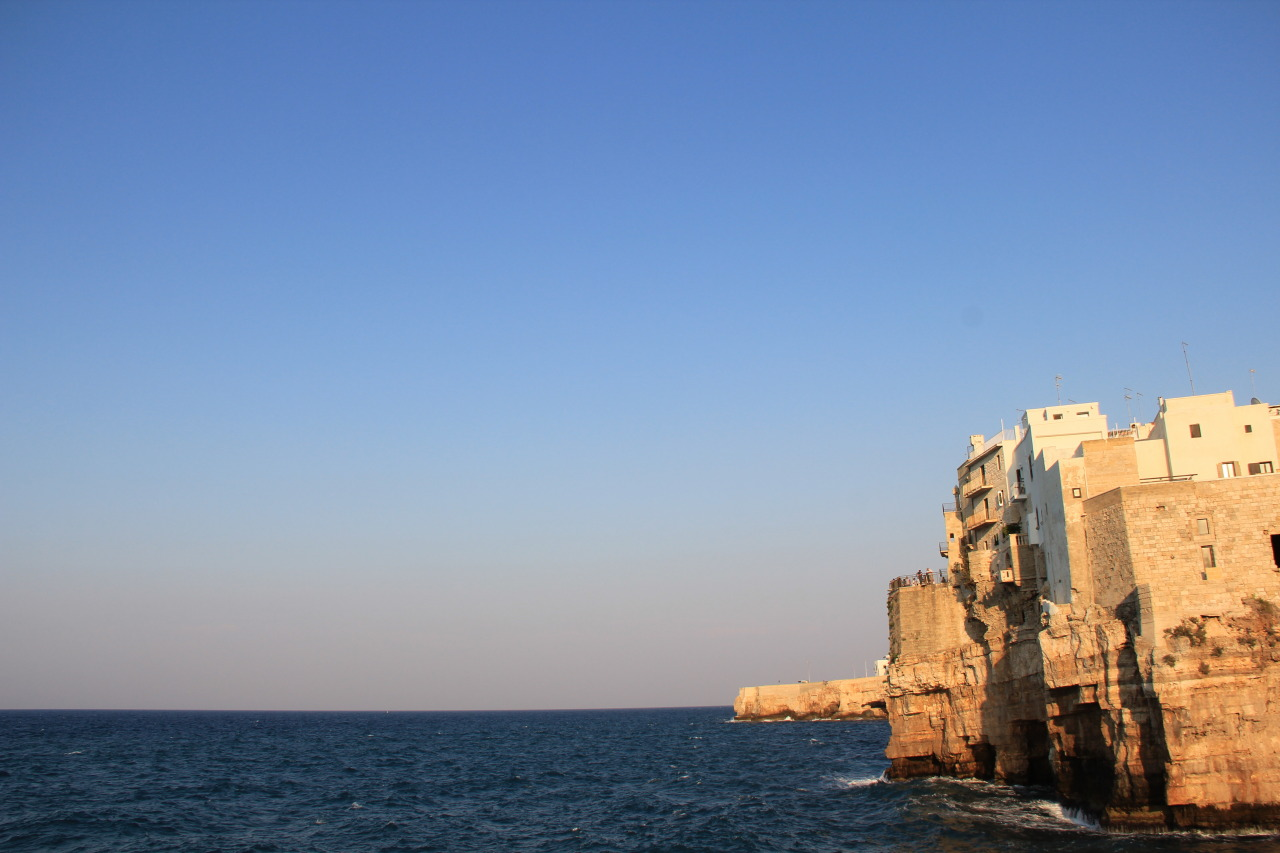
\includegraphics [width=0.3\textwidth]{../Bilder/Sommer2012/56.jpg}}\quad
   \subfloat{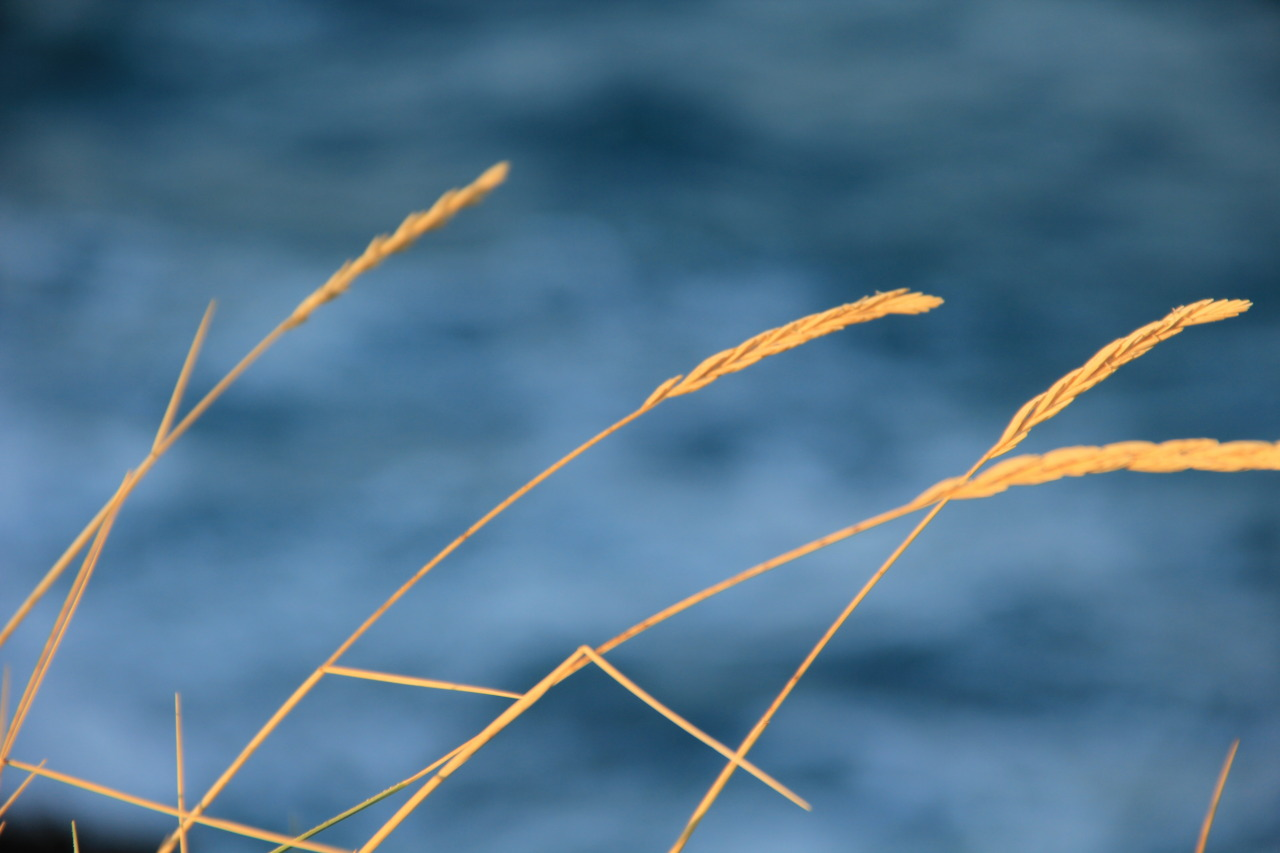
\includegraphics [width=0.3\textwidth]{../Bilder/Sommer2012/57.jpg}}\quad
   \subfloat{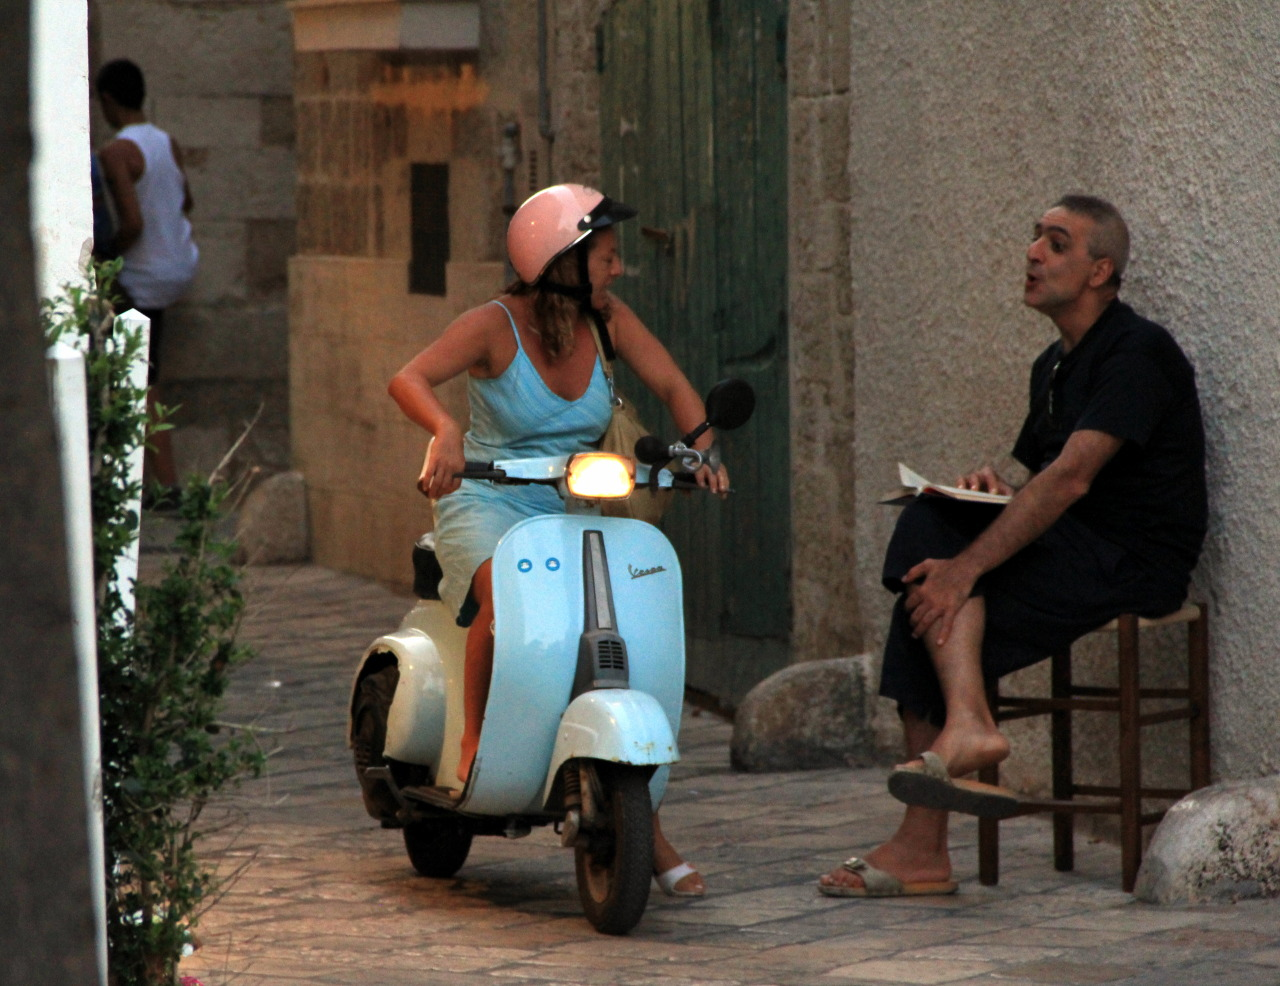
\includegraphics [width=0.3\textwidth]{../Bilder/Sommer2012/58.jpg}}\quad
   \caption[Polignano al Mare]{Polignano al Mare}
\end{figure}

Zur�ck auf dem Posten waren die anwesenden Polizisten zwar sehr Hilfsbereit, konnten jedoch in etwa so gut Englisch wie ich Franz�sisch.
Vor allem das Diktieren der geklauten Gegenst�nde wurde zu einem Ratespiel \`a la Tabu, Montagsmaler oder \glqq Ich seh etwas was du nicht siehst \grqq.
Trotz allem verlief das Ganze relativ schnell und nach 3/4 Stunden waren wir auf dem Weg nach Monopoli.
Unsere Wasservorr�te waren arg strapaziert worden und wir mussten noch Linsenmittel f�r Chantal sowie endlich ein Kabel f�r Jack finden.
Nach mehreren Eurospars, Lidl und anderen Supermercati hatten wir zwar alles erdenkliche gefunden, vom Linsenmittel fehlte aber noch jede Spur.
Gegen den Abend wurde es richtiggehend k�hl.
Ja, unglaublich aber wahr, Chantal verkroch sich schon bald unter eine Decke und wir a�en unsere mittlerweile gut bekannten Pasta.
Der Besuch eines Bewohners des Campinglatzes der mehrere Jahre f�r Rolex in Genf gearbeitet hat und erkundigte sich wie man Ricola richtig ausspricht, sorgte f�r eine willkommene Aufheiterung.

\subsection{13.08.2012 Neue Woche neues Gl�ck}

\begin{wrapfigure}{L}{0.45\textwidth} 
  \begin{centering}
    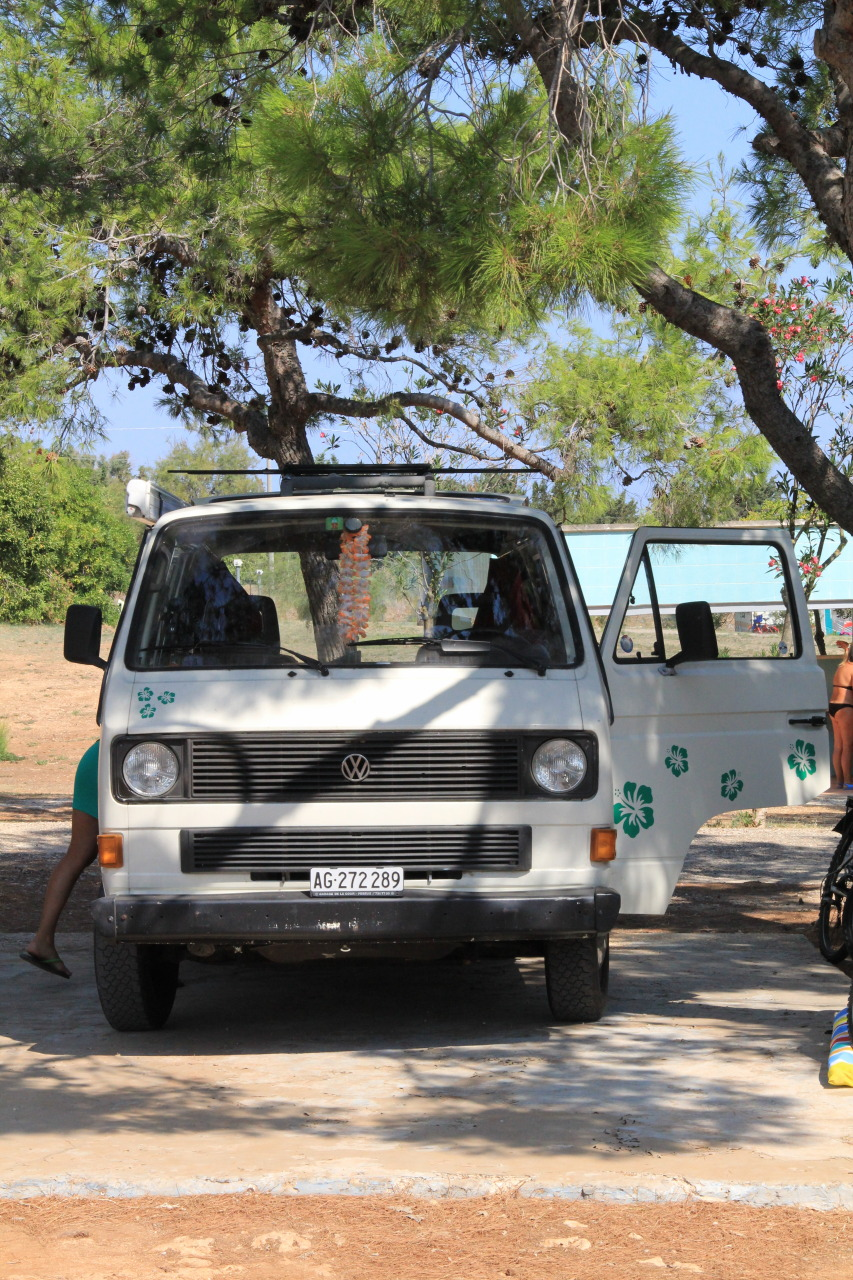
\includegraphics[width=0.4\textwidth, height=5cm, keepaspectratio]{../Bilder/Sommer2012/60.jpg}
    \caption{Campingplatz San Stefano}
  \end{centering}
\end{wrapfigure} 

Die neue Woche brachte zuerst einmal etwas Neues: Regen! Kurz nach dem aufstehen fielen fette Regentropfen vom Himmel.
Die Markise ausgefahren und wir konnten trotzdem gem�tlich zm�rgelen.
Wir nutzten die nasse Pracht gleich um die Scheiben von Jack zu reinigen.
Gut verteilt ist halb geputzt.
Durch das Wetter fiel der Strandtag buchst�blich ins Wasser.
Wir zogen uns noch einmal in den Bus zur�ck schauten Filme uns ich begann mit dem Studium des Kroatien-Reisef�hrers, welcher die Vorfreude betr�chtlich steigerte.
Mitte Nachmittag besserte sich das Wetter und wir begaben uns per Bike nach Monopoli.
Am stadteigenen Strand h�pfte Chantal kurzerhand ins Wasser, w�hrend dem ich mich �ber die fehlenden Badehosen meinerseits �rgerte.
Beim Streifzug durch die Stadt um das langersehnte Linsenmittel zu finden trafen wir auf eine vorz�gliche Gelaterie, welche man nat�rlich nicht einfach links liegen lassen konnte.
Schlussendich wurden wir dann endlich f�ndig und eine letzte Pendenz der Diebstahlliste konnte abgehackt werden.
Chantal hatte endlich ihr Linsenmittel.
Ein Grund zum Feiern! Wir lie�en uns den Caipiroska und den Latino-Americano die Kehle herunter rollen und fanden schon bald darauf ein kleines Feines Restaurant das Chantal mit Fisch versorgen konnte.
F�r mich wurde ein weiteres Mal die Spaghettipresse angeworfen und der Fischer mit der Suche nach Meeresfr�chten beauftragt.
Die wiederum dunkle Fahrt zur�ck zum Camping verlief dann reibungslos

\subsection{14.08.2012 Ohne Drucker keine Fahrt}

\begin{wrapfigure}{R}{0.45\textwidth} 
  \begin{centering}
    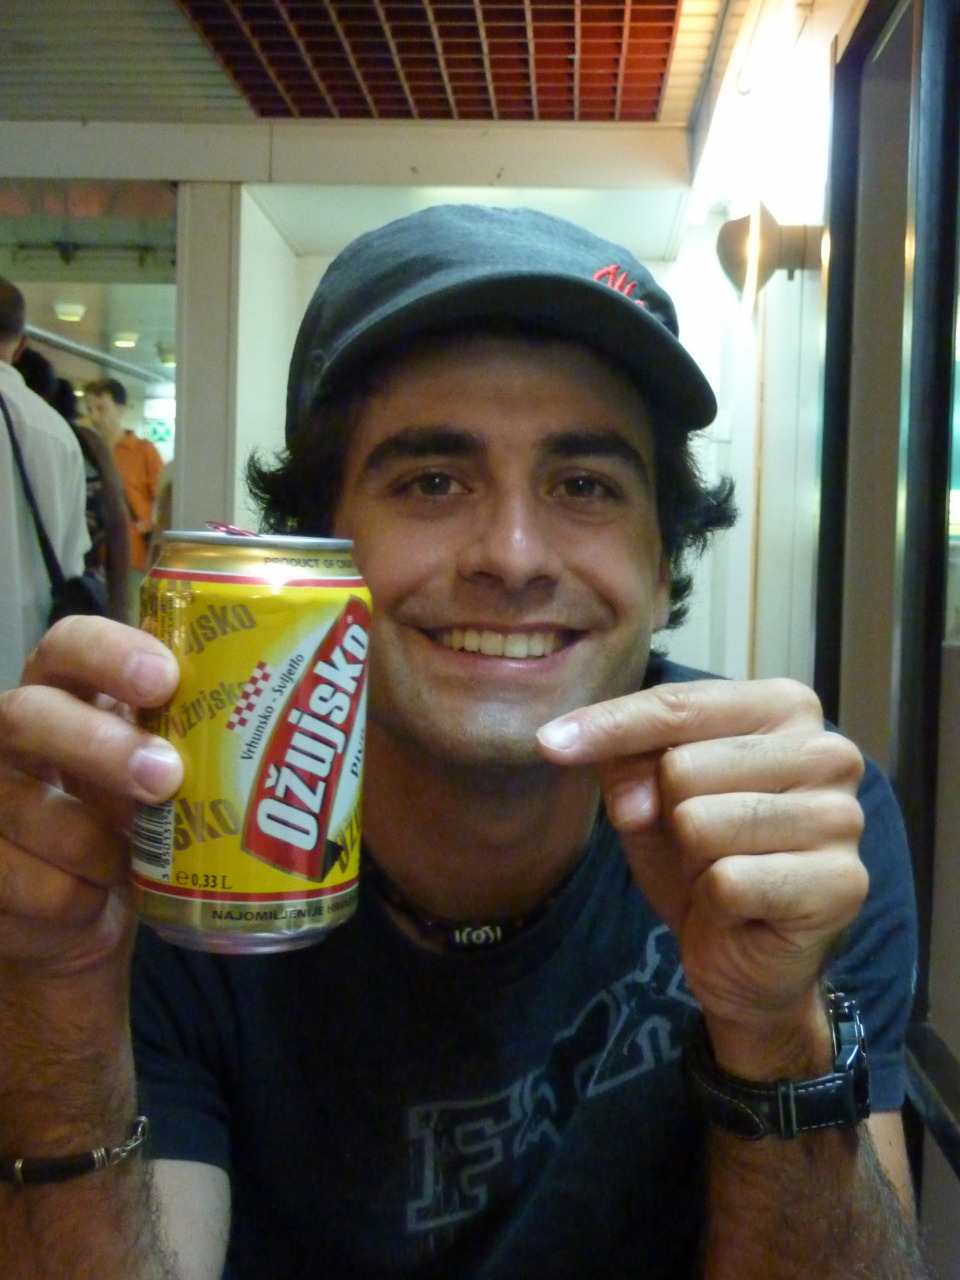
\includegraphics[width=0.4\textwidth, height=5cm, keepaspectratio]{../Bilder/Sommer2012/62.jpg}
    \caption{Erster kulturelle Kontakt mit Kroatien}
  \end{centering}
\end{wrapfigure} 

Auch heute wurden wir nicht wie gewohnt durch Sonnenstrahlen geweckt, sondern eher durch Wolken und kurze Schauer. Die Fahrt nach Bari, die Stadt, welche laut Reisef�hrer ein Chaos sein soll, stand heute auf dem Fahrplan. Freude herrscht. Zuerst musste jedoch noch einmal das F�dli ins Meer gehalten werden. Nach dem Auschecken besuchten wir den nahegelegene Strand, welcher jedoch nicht gerade eine Augenweide war. Scharfe Klippen verunm�glichten ein Liegen und um zum Wasser zu kommen waren Ninja-Kenntnisse von Not gewesen um den Rasiermesserscharfen Steinen auszuweichen. Diese Umst�nde verhinderten nicht einen wahren Menschenstrom, welcher es sich irgendwie (wie auch immer) am Strand bequem machte. Wir zogen weiter gen Norden und fanden beim zweiten Anlauf einen herrlichen Sandstrand mit Bistro.
Beim durchst�bern eines zweiten Reisef�hrers blieben uns glatt die bestellten Orechiette im Hals stecken. Laut Aussage des Autors, war das Einreisen nach Kroatien nur mit Pass, nicht mit ID m�glich. So soll es jedenfalls f�r Schweizer sein. Es stellte sich heraus, dass dieser Reisef�hrer um einiges aktueller war als der andere. Hoppla. Ich hatte meinen Pass zu Hause gelassen, da es laut TCS nicht n�tig sei diesen mitzunehmen und den Pass von Chantal hatte Giovanni und seine Crew nun irgendwo in Palermo. Das einzige was uns �brig blieb war zu hoffen das sich der sich als �usserst kompetent ausgebende Autor t�uscht.
Die Fahrt nach und durch Bari verlief v�llig Problemlos. Der Hafen war gefunden, jedoch war das B�ro bis 18:30 geschlossen. Und ohne den Zettel war die Zufahrt zum Hafen nicht erlaubt und wurde durch grimmig Beamte der Guardia di Finanza kontrolliert. Die einem Labyrinth �hnelnden Altstadt war schnell durchquert und ein Shoppingparadies er�ffnete sich vor Chantals F�ssen, welches sogleich erkundet werden wollte. Ich ging auf die Suche nach einem WLAN um die unklare Situation betreffend Einreise zu kl�ren. Es zeigte sich, dass der TCS wirklich nichts von einem Pass erw�hnt. Also d�rfte soweit alles in Ordnung sein. Bosnien-Herzegowina verlangt jedoch einen Pass. Diese m�ssen wir durchqueren, wenn wir Kroatien auf dem Landweg nach Norden durchfahren wollen. F�hren bieten hier jedoch eine Alternative.
Kurz vor sieben fanden wir eine betrechtliche Schlange vor dem Schalter. Auch eine Stunde sp�ter war die Schlange vor uns noch unver�ndert. Nach hinten zeigte sie jedoch einen klaren Aufw�rtstrend, was die Wartezeit betraf. Ich klingte mich aus der Warteschlange aus um etwas essbares zu besorgen und den Wasserhaushalt wieder in Balance zu bringen und auch nach dem zur�ckkommen mit Hot Dog das gleiche Bild. Jetzt jedoch waren schon etliche Personen damit besch�ftigt den Drucker f�r die Tickets zum laufen zu bringen. Leider noch ohne Erfolg. Uns besch�ftigte noch eine weitere Frage: Warum standen alle Wartenden mit Gep�ck in der Schlange? Auch nach mehrmaligen Erkundigen konnte uns keiner eine Antwort daraufgeben ob wir am richtigen Ort anstehen. Hinter uns stand ein P�rchen aus Bosnien an, mit denen wir schnell ins Gespr�ch kamen. Beide sprachen relativ gut Englisch und erz�hlten uns etwas �ber Kroatien, Bosnien, Ihre Reise nach Italien (14 Stunden Shoppingtrip, crazy) und die Politische Lage in ihrem Land. W�hrend dem spannenden Gespr�ch konnte der Drucker �berzeugt werden Tickets auszuspucken und kurz nach 20:00 waren wir an der Reihe und nat�rlich wurde der Fahrzeugausweis verlangt, welcher sich auf dem Parkplatz im Bus befand. Los gerannt und diesen geholt und wild fluchend mit allerlei Zettel versehen mit Barcodes versuchten wir den Hafen zu entern. Vergebens. Das Schiff stand zwar in Sichtweite, jedoch wurden wir zu einem 3 km entfernten anderen Tor geschickt. 3 km Richtung Westen um Nachher wieder 3 km nach Osten zu fahren um an der anderen Seite der Barriere (vor welcher wir gerade standen) aufzutauchen. Anstehen f�r Zoll und andere Jacks, eh Checks. Am Viertel ab 9 hatten auch wir es geschafft und der Bus war im Bauch der kleinen F�hre verstaut. Die Kabine war dann schnell gefunden und mit einer Stunde Versp�tung ging die Fahrt nach Kroatien los. Das erste Kroatische Bier wurde genossen, zu Essen gab es nichts mehr. Kurz darauf d�sten wir ein...

\subsection{15.08.2012 Dubvronic}
Um 5:30 klingelte der Wecker, Fr�hst�ck gab es von 6-7. Das Schiff holte die st�ndige Versp�tung problemlos auf und schon w�hrend dem zerkleinern des Toasts kam die \glqq Skyline \grqq von Dubrovnic in Sichtweite. Nach dem anlegen meinte ein Kroatischer Zollbeamte, dass uns der Kleber mit dem ber�hmten \glqq CH \grqq fehle. Da wie jedoch Schweizer seien vertraue er darauf, dass wir einen solchen noch beschaffen werden. Bei Italienern sei das eine ganz andere Geschichte. F�gte er noch lachend hinzu.
Der Camping Solitude war schnell gefunden und die nette multilinguale Empfangsdame versprach uns einen Platz, der jedoch erst ab 10:00 zur Verf�gung stand. Wir verbrachten die Zeit d�send auf dem Parkplatz.
Nach dem Beziehen des Platzes, stand auch schon die erste Velotour auf dem Programm. Richtung Altstadt sollte es gehen. Nach einer halben Stunde erreichten wir diese durchgeschwitzt. Wir waren nat�rlich ein weiteres Mal in der gr�ssten Hitze aufgebrochen. Die Altstadt von Dubrovnic war an den Menschenmassen zu erkennen. Man k�nnte meinen es sei Stadtfest. Wir fl�chteten schnell in die Seitengassen und an den wundersch�nen Hafen, um die Beine ins Meer zu halten, welches Glasklar die Hafenmauern umsp�lte. Nach einer halben Stunde wurde ich schon das erste Mal ein Opfer von einer fiesen Krebs-Attacke. Diese kleinen Biester kletterten die Senkrechte Mauer m�helos empor. Nach einem kurzen Abstecher im Nike Store ( Wie war der Umrechnungsfaktor Kuna-CHF?) ging es hinauf auf den H�gel neben der Stadt um die wundersch�ne Aussicht zu geniessen. Eine Gondelbahn bringt einem m�helos hinauf und die Sicht ist atemberaubend. Wir entschlossen heute selber zu kochen und deckten uns nach der R�ckfahrt im Campingeigenen Laden mit Wienerli und Thunfisch und Salat ein. Die Wienerli waren nicht gerade der Renner der Rest verschwand jedoch �usserst schnell in unseren Magen. Chantal bewiess ihr K�nnen an der Waschmaschine und stockte unsere Kleidervorr�te wieder auf. Zeit zum Schlafen...

\subsection{16.08.2012 Erste Schnorchelversuche und Mauerwanderung}
Nach dem anstrengenden sportlichen Tag gestern war heute wiedermal ein Strandtag angesagt. Die nahrhaften Gipfeli und die riiiesige Wassermelone zum Zmorgen waren ein guter Start in den Tag. Sch�n ausgeschlafen und gest�rkt machten wir uns auf den Weg zum Campingstrand. Dieser war ziemlich �berf�llt aber sehr sch�n: glasklares Wasser und eine sch�ne Aussicht auf Inseln, die sch�ne Br�cke vor Dubrovnik und die Gebirgsz�ge. Wir verbrachten den Nachmittag mit Faulenzen und Baden. Wir versuchten uns auch im Schnorcheln (bei einigen sah man nur noch viiele Haare und der Schnorchel oberhalb vom Wasser ;)), doch ausser einigen Albinofischen sahen wir nicht viel spannendes (kein riesen Tintenfisch wie in Koriska :)).

Um 4 Uhr gings zur�ck zum Camping und dann mit den Velos nach Dubrovnik. Diesmal war es etwas angenehmer und nicht mehr so erdr�ckend heiss wie gestern. Dort angekommen, war unsere Mission: der Spaziergang �ber die ber�hmte Stadtmauer. Touristen hatte es immer noch zu gen�ge und wir mussten nur schon f�r die Tickets um auf die Stadtmauer zukommen, anstehen. Aber es ging ruchzuckzackzack und es lohnte sich wirklich. Die Aussicht von der Stadtmauer auf die Altstadt und vor allem auf das Meer und
die vorgelagerten Inselchen war traumhaft. Es ging 2 Kilometer (ungef�hr eine Stunde) stegeli ufe und stegeli abe, was abenteuerlich und anstrengend war. In jedem G�sschen und auf Dachterrassen entdeckten wir viele herzige Restaurants, von welchen ein feiner Duft zu uns wehte, was ziemlich gemein war, da wir richtigen Kohldampf hatten. Daher sprinteten wir nach unserer Wanderung direkt in ein feines Restaurant. Es gab weisses Risotto mit Garnelen, Spaghetti mit Meeresfr�chten und Muscheln,
Tintenfische, Schrimps und Fisch ... hmmmm das war lecker!:) Nach dem Essen rugelten wir zur�ck zum Camping wo ich schnurstracks in einen Tiefschlaf fiel. Stefan schrieb noch fleissig an unserem Tagebuch, bevor es dann auch hiess: dobra vecer.

\subsection{17.08.2012 Korcula}
Heute war Aufbruchstimmung. Die Insel Peljesac und die Insel Korcula stand auf unserem Programm. All unsere sieben Sachen gepackt, machten wir uns auf den Weg und schon bald waren wir aus Dubrovnik heraus, �ber die wundersch�ne Br�cke vor Dubrovnik und auf der K�stenstrasse. Diese verlief kurvenreich und mit einer atemberaubenden Aussicht auf das Meer und die zahreichen Inselchen. Die Fahrt durch die Insel Peljesac war sehr gem�tlich; viel Wald, einige D�rfer und ein paar Burgen mit ihren riesigen Festungsmauern. Die Stadt Ston hat sogar die l�ngste Festungsmauer (5km) von Europa. Zuerst wollten wir auf einem kleinen abgelegenen Campingplatz in Trpanj �bernachten, doch dann entschieden wir uns sogleich nach Orebic, welches am Ende der Insel liegt und Ausgangspunkt f�r die Insel Korcula ist, zu fahren.
Wir hatten Gl�ck und haben ohne langes Warten eine F�hre erwischt. Jupii, das Insel-Hopping kann beginnen;) Schon nach ungef�hr 20 Minuten waren wir in Korcula. Ich habe im Reisef�hrer gelesen, dass Korcula auch sehr beliebt bei den Einheimischen ist, da das Klima sehr mild ist und die Winde Bora und Jugo nicht so stark sind (Die Bora kann sehr gef�hrlich sein, da es schon vorgekommen ist, dass Autos von der K�stenstrasse regelrecht weggewindet wurden). Doch diese Information war irgendwie nicht so wahrheitsgetreu, denn schon auf der F�hre erblickten wir so viele Wind- und Kitesurfer wie noch nie, die ziemlich schnell herumflitzten und in Korcula angekommen, windete es uns fast davon. Wir fuhren in die Stadt Korcula herein, schlenderten durch die Alstadt und g�nnten uns eine Pizza in einem Restaurant direkt am Meer. Dann machten wir uns auf nach einem nahegelegnen Camping, wo wir sofort einen Platz beziehen konnten. �berraschung! Unser Nachbarauto war ein hellblauer VW-Bus aus Solothurn, welchen wir auf dem Camping in Dubrovnik schon gesehen hatten. Und kaum ausgestiegen, kam deren Besitzerin schon auf uns zu und plauderte los �ber ihre Reservierungsmiseren und die beschwerliche Reise nach Dubrovnik. Zudem zeigte sie uns die "sch�ne" Innenausstattung des VW-Buses (brauner Teppich). Doch am besten gefielen mir die hellblauen Delphine, welche auf den Bus gesprayt waren ;) Sie gab uns noch ein paar gute Tipps wie z.B das Insel-Hopping spart enorm Zeit. Diese Aussage k�nnen wir nach einem weiteren F�hrentripp, �ber welchen morgen berichtet wird, bereits widerlegen. Nach diesen vielen Informationen gingen wir kurz an den Strand. Doch wir hatten fast ein bisschen kalt, da es so windete wie noch nie..auf dem windstillen Korcula. Zum Znacht gab es Suppe, Chips und ein etwas speziellen Wein aus der Region (in einer Cola-Flasche;)).

\subsection{18.08.2012 Wie kommen wir von dieser Insel weg?}
Der bef�rchtete Hang-over vom Inhalt der frisch erworbenen Cola-Flasche blieb zum Gl�ck aus. Wir standen schon um 8:00 auf um die F�hre nach ... um 10:30 sicher zu erreichen. Nach dem Verabschieden der Kroatien-Spezialisten waren wir schon auf dem Weg zum Hafen. Naja, w�ren, wenn da nicht eine 250 Meter lange Kolonne ist, welche denn Weg in den Hafen verstellt. Jack schloss hinten an und wir wanderten der Kolonne entlang Richtung Ticket Office, dass uns sogleich mittteilte, dass die erste F�hre ausgebucht sei. Die n�chste Fahre um 16:30! Ratlosigkeit machte sich breit. Insel-Hopping ist ja sch�n und gut, aber ohne F�hre mit einem Auto relativ m�hsam. Fahren ist auf jeden Fall besser als hier bl�d herum stehen und so beschlossen wir den Weg nach Vera Luka unter die R�der zu nehmen. Eine wundersch�ne Strasse f�hrte �ber die ganze schier unbewohnte Insel und schon bald tauchten wir von den Bergen hinab in die gr�sste Stadt der Insel.
Split war in Sicht und mit der Stadt auch die Tafelberg �hnlichen Erh�hungen im Hintergrund. Was zus�tzlich auffiel, war die Verf�rbung der Luft, hervorgerufen durch etliche Feuer rund um Split. Seit l�ngerer Zeit waren wieder einmal Hochh�user in Sicht und wir beschlossen, dass wir Split nicht n�her anschauen wollten und gleich Richtung Trogir weiterziehen wollen.
Dort angekommen war der erste aufgesuchte Camping in Stadtn�he leider voll. Es wies jedoch ein Schild auf einen anderen hin, denn wir sogleich aufsuchten. 1.2 km vor dem Camping war es dann vorbei mit Teerstrasse und ein unbefestigter Weg breitete sich vor uns aus. Los ging die wilde Fahrt, welche durch einen winzig kleinen sehr freundlichen Campingplatz mit angeschlossenem Restaurant belohnt wurde. Der Stellplatz war zwar selbst f�r unseren kleinen Bus sehr eng, jedoch mit direkter Sicht auf das Meer.  Zum Abendessen gab es Dalmatinischer Rohschinken und je 300 gr. Scampi mit Pommes Frites. Herrlich.
Danach fiel ich m�de ins Bett, w�hrend Chantal noch kurz die Berichte auf Vordermann brachte.

\subsection{19.08.2012 Strandtag}
Um kurz nach acht trieben uns die schon stark erh�hte Temperatur und das Brot das von 8-9 verkauft wird aus den Federn. Chantal besorgte uns ein reichlich gedeckter Fr�hst�ckstisch. Ein kurzer Ausflug unter die Dusche und bald schon stand der sehr kurze Spaziergang zum Strand an. Das wunderbar klare Wasser und die hohen Temperaturen verfehlten ihre Wirkung nicht und schon bald schwammen wir mit Go Pro, Schnorchel und Taucherbrille in der herrlichen Bucht. D�sen und Lesen ergaben dann schnell Hunger und das Restaurant, welches uns am Vorabend mit Essen versorgte versuchte mit Scampis �ber dem Feuer gebraten die G�ste zu verf�hren. Wie unschwer zu erraten ist funktionierte diese List bei uns perferkt und nur vom Unterbewusstsein gesteuert fanden wir uns vor dampfenden Nudeln mit Scampis wieder. Eigentlich wollten wir wenn m�glich noch Trogir besichtigen, was jedoch dank des sch�nen Strandes eher morgen geschehen wird.
Wie man leicht erkennen kann, eignen sich Strandtage nicht gerade dazu viel und interessantes zu berichten. Vielleicht noch dass: Unser Cola-Flaschen-Wein hat die warme �berfahrt in der F�hre nicht gut �berstanden. Der Geschmack hat sich zwar nicht ver�ndert, die Auswirkungen hingegen schon.

\subsection{20.08.2012 Fahrt �ber eine total andere Insel}
Wir werden die wundersch�ne Aussicht, welche jedes Morgenessen hier untermalt vermissen. Trotzdem hiess es heute weiter ziehen Richtung Norden. Auch diese Fr�hst�ck wurde durch feine B�ckerei-Leckerbissen aufgem�belt. Dieses Mal war es ein Apfelstrudel und zwei Berliner (einer mit Nutella, Gruss an Susi). Bevor wir nach Trogir reinfahren konnten, mussten wir noch etliche H�rden �berwinden. Zuerst mussten wir den schmalen Weg meistern. Chantals Abdr�cke der Fingern�gel sind immernoch am "Angsthasengriff" sichtbar. Als zweites mussten wir einkaufen, �berhaupt kein Problem, da ein Market auf dem Weg lag. Das dritte Problem bestand darin, nach Trogir zu kommen.Das malerisch gelegene St�dtchen bietet die einzige Br�cke zu der Insel, auf der wir uns befanden. Entsprechend beliebt ist dieser Ort bei den Autofahrern. Nach etwa einer Stunde Stop and Go haben wir die zwei Br�cken erreicht und fanden noch kurz Zeit mit einem Schweizer Ehepaar zu quatschen, welche sich �ber Jack freuten. Ein Parkplatz war dann schnell gefunden und auf ging es die Stadt und Ihre Schmuckgesch�fte zu erkunden. Eine wundersch�n gelegene Stadt, die jedoch irgendwie wie jede andere kroatische Stadt aussah, die wir bis anhin besuchten. Massen von Touristen wuselten durch die Gassen und die ganze Altstadt bestand aus Restaurants. Nach einer feinen Pizza ging es Richtung Norden.
Kurz vor der Autobahnauffahrt �berholten uns wieder einmal L�schflugzeuge um in Sisiphusarbeit den nahe brennenden Wald zu l�schen. �berhaupt sieht man sehr viele schwarze, runtergebrannte Stellen wenn man durch diese sehr trockene Gegend f�hrt. Das Bezahlsystem funktioniert sehr �hnlich wie das in Italien, nur moderner schneller und freundlicher. Auch das Chaos nach der Bezahlstelle h�lt sich stark in Grenzen. Es fuhren im allgemeinen nur wenige Fahrzeuge auf der gut ausgebauten Autobahn. Die Vegetation �nderte sich schlagartig, als wir auf die Insel Pag auffuhren. Nix mehr Gr�nes, es war eher eine Mondlandschaft als das bekannte Inselartige, dass uns jetzt schon �ber eine Woche begleitete. Das herrlich blaue Wasser bildet einen wunderbaren Kontrast zu den hellen steinigen Weiten.
Unser erster angesteuerte Campingplatz lag ganz am Ende der Insel und gegen Ende eben dieser wurde die Strasse immer spannender mit Kuppen �berzogen die dem Fahrer grosse Freude bereiteten. Auch dieser Platz lag wieder wundersch�n an einer einsamen Bucht und am Ende einer engen Strasse. Als wir dem Platz entlang fuhren, wurde uns jedoch schnell klar, dass hier nichts mehr zu machen ist. Voll. Leider best�tigte sich dieser Verdacht und der nahegelegene Alternativplatz bot leider weit und breit
keine Verpflegungsm�glichkeit, geschweige denn Elektrizit�t. Also fuhren wir auf dem Inselr�cken zur�ck nach Novalja, wo sich einer der Top 10 Pl�tze Kroatiens befinden soll. Der Platz ist gigantisch. �ber 1200 Stellpl�tze eigene Check in Spur in der Anfahrtsstrasse, Sportcenter und und und... Wir waren zuerst nicht gerade begeistert, jedoch mussten wir unsere Meinung sehr schnell �ndern. Sch�ner Strand, sehr sch�ne Sanit�re Anlagen, alles passt. Nach dem wir wieder einmal selber gekocht hatten
(Sweet \& Sour mit Reis und Poulet, dazu Maissalat) fielen wir M�de aber gl�cklich ins N�scht.
Da wir auf dieser Reise einen GPS Tracker mitf�hren kennen wir ausnahmsweise (ein kleines Leiden von Jack) die zur�ckgelegten Kilometer. Wir haben bis zum heutigen Tag 2245 km zur�ckgelegt. Ohne auf Probleme gestossen zu sein. Wir hoffen, dass es auch auf dem Rest der Reise so bleiben wird.

\subsection{21.08.2012 Annehmlichkeiten eines Luxus-Campingplatzes}
agwach verschliefen wir gekonnt. So standen wir erst gegen 10:00 auf, was wir auch unserem schattigen Pl�tzchen verdanken konnten. Danach ging ich einkaufen und besorgte das Passwort f�r das streng gesch�tzte Platz eigene WLAN. Damit konnten wir uns wiedereinmal �ber die geschehenen Dinge in der Welt informieren und Chantal bekam die wunderbare Nachricht, dass sie die n�chste Zeit viel Spass an der Franz�sischen Sprache haben darf. Als die Sonne ihren h�chsten Stand erreichte begaben wir uns an den Strand. Dieser war wie alles auf diesem Platz einfach gigantisch.  Jede erdenkliche Wassersportart wurde angeboten, bis zum Wasserstrahl betriebenen Raketenrucksack.

Als wir eine feine Garstufe erreicht hatten, war es Ap�rozeit und danach wurden die Duschen aufgesucht. Die Fahrt an den endlosen Caravan-Stellpl�tzen vorbei war eindr�cklich und wenig sp�ter kam schon das D�rfchen direkt am Wasser ins Sicht. Am Eingang zum Dorf warteten schon die Restaurants mit montierten Spanferkel auf die zahlende Kundschaft. Das ausgesuchte Restaurant konnte vollends �berzeugen. Auf dem Weg dorthin war ich mir noch sicher heute garantiert kein Fisch zu essen. Dieser Vorsatz
verschwand dann aber schneller als er aufgetaucht war beim Blick auf die Speisekarte. Schlussendlich fanden Miesmuscheln und Risotto mit Meeresfr�chten ein weiteres Mal den Weg auf den Tisch. Chantal verschonte die �berfischten Gew�sser mit ihrer Wahl und suchte sich Teigwaren mit Tr�ffel aus. Nach dem Essen war auf der Strandpromenade dir Party voll im Gange und auch die Gesch�fte lockten Chantal ein weiteres Mal mit ihren hochwertigen Artikel an.
Auf dem Zeltplatz angekommen herrschte auch da in einem der vielen Restaurants noch Oktoberfeststimmung. Bald darauf legten wir uns auf die Ohren und h�rten f�r die n�chsten Stunden dem Kopfkissen zu.

\subsection{22.08.2012 Rab - Zeit um die Insel zu wechseln}
Heute wollten wir Dea und Lukas besuchen. Deas Familie besitzt eine wundersch�ne Ferienwohnung oberhalb von Rab mit einem atemberaubenden Ausblick �ber das St�dtchen. Zuerst mussten wir jedoch von Novalja auf Pag zur�ck auf das Festland um dann wiederum auf die n�chste Insel, eben Rab zu kommen. Kurz vor zw�lf machten wir uns auf den Weg und weil beide ben�tigten F�hren im 20 min Takt fuhren kamen wir kurz darauf schon in Rab an. Eigentlich haben wir uns f�r etwa 18:00 Uhr angemeldet und die
beiden genossen noch das glasklare Wasser auf der Insel Frkanj. Chantal besorgte die Geschenke f�r Silas (ihr G�ttibueb) und ich versuchte Impressionen mittels Fotoapparat auf die Harddisk zu schreiben. Der kleine Hunger meldete sich, hatte jedoch auch hier kaum eine Chance gegen die Flut der Restaurants. Es war h�chste Zeit sich mit Hilfe des Wassers abzuk�hlen. Rab besitzt auf der einen Seite eine wundersch�ne Uferpromenade, welche zum Baden einl�dt. Kaum dort angekommen und die ersten Krebse
und Fische beobachtet meldeten sich unsere beiden Gastgeber, dass sie auf dem R�ckweg von der kleinen Insel seien. Wir trafen die beiden im Hafen und beschlossen die Abendsonne am vorher besuchten Stadtstrand zu geniessen und erst nachher mit Jack zur besagten Wohnung zu fahren. Der Weg da rauf war steil und eng und die beiden organisierten gar extra einen Parkplatz f�r den Bus. Wir durften ein eigenes Zimmer beziehen mit eigenem Bad. Welch Luxus nach fast drei Wochen Camping. Dea hatte
nat�rlich ein paar gute Vorschl�ge f�r das Nachtessen und dank ihrem kroatisch verschwanden schnurstracks die \glqq Reserviert \grqq T�felchen von den letzten Tischen im Restaurant und wir genossen ein herrliches Abendessen zu viert.

\subsection{23.08.2012 Die Liebesinsel ;)}
Wieder einmal ein richtiges Bett, juhuu :) Wir kamen fast nicht aus den Federn, als um 8 Uhr der Wecker klingelte. Und dies obwohl uns schon um 6 Uhr ein Ger�usch weckte; kiikerikiii, kikerikii. Kaum aufgestanden, war schon das Fr�hst�ck parat: feine M�esli, Brot, Marmelade, Wassermelone...alles was das Herz begehrte, hmm:). Und all dies konnten wir mit einer herrliche Aussicht auf Rab und vorgelagerten Inselchen geniessen. Eine dieser Inseln war die Insel Frkanj, die sogenannte Liebesinsel; welche wir heute besuchen wollten. Nach dem gem�tlichen Fr�hst�ck packten wir unsere Standsachen und machten uns auf den Weg zum Hafen. Dort wartete schon unser Taxiboat. Die Fahrt nach Frankj war herrlich und dort angekommen, wussten wir, dass es noch viel herrlicher wird:) Glasklares Wasser, einen sch�nen Pinienwald und ein super Restaurant erstreckten sich vor uns. Wir suchten uns ein lauschiges Pl�tzchen im Schatten aus und machten schon bald ein Sprung ins Wasser...wow, wundersch�n wares! Den Rest des Tages verbrachten wir mit: schwimmen, schnorcheln, faulenzen, spektakul�ten Steinm�nnli bauen (g�ll Steff:)) und essen. Zu Mittagessen gab es feine Meeresfr�chte und Fleisch (niemand traute sich an das Spannferkel). Auch diesmal bekamen wir dank Dea einen eigentlich reservierten Spitzenplatz. Nach dem Essen verfielen wir in einen Tiefschlaf. Doch wir konnten uns dann doch noch aufraffen f�r einen weiteren Schwimmtrip zum Restaurant und f�r einen Misch-masch und Sonnenaufgang, welcher sich dann leider als Sonnenuntergang herausstellte.  Das Taxiboat zur�ck haben wir knapp noch erwischt. Im Hafen angekommen, waren wir alle ein bischen plemplem und schlenderten den Hang hinauf zu Deas Wohnung. Dort ging es ruckzuckzackzack ans Kochen und schon bald konnten wir ein feines Nachtessen mit Spaghetti, serbischem Salat und sehr sehr gutem Wein mit wundersch�ner Aussicht geniessen. Die farbige Disco-Beleuchtung zog uns dann noch zur down town von Rab;) Nach einem Stadtrundgang entschieden wir uns schlie�lich f�r eine Bar, wo es Mojito, Wasser und Eistee gab (jemand hatte schon zu viel von dem guten Wein getrunken;)). Es war ein gelungener Ausklang f�r einen wundersch�nen Tag!
\subsection{24.08.2012 Wir m�ssen weiterziehen}
Auch wenn es noch so sch�n auf Rab gewesen ist, war trotzdem die gekommen um weiterzuziehen. Dea und Lukas entschieden sich die Gelegenheit f�r eine Besuch der Str�nde um Lopar. Wir parkten den Bus vor dem F�hrehafen und wollten eigentlich gleich Tickets f�r die F�hre kaufen. Das Ticket-Office �ffnete seine Fenster jedoch erst um 13:00. Der Bus stand jedenfalls so nahe an der Poleposition wie noch nie, was einem garantierten Platz auf der F�hre gleichkommt. Mit dem Fahrzeug der beiden ging es dann auf Strandsuche. Nach kurzer Fahrt empfing uns ein Parkticketverk�ufer im weiten Wald. Dieser wollte Geld f�r ein Ticket, welches die Einfahrt in seinen Parkplatz erm�glicht. Es war nicht gerade ein Parkplatz im klassischen Sinne. Viel eher ein bewaldetes St�ck Land, durchzogen von etlichen Strassen und Wege, an denen sich �berall Ecken und Pl�tzchen f�r das Abstellen der Fahrzeuge finden lies. Um an den Strand zu gelangen war dann ein l�ngerer Marsch notwendig und wir f�rchteten uns schon vor m�glichen Nakedei, die an diesen Strandabschnitten geduldet wurden. Nach den ersten vorsichtigen Blicken gab es Entwarnung und wir trauten uns n�her an die Bucht, welche durch grelles Kindergeschrei mit Leben erf�llt worden ist. Die ziemlich grosse Bucht bot die M�glichkeit 200 Meter �ber feinsten Sandboden ins Meer heraus zu waten ohne das der Nauchbabel auch nur in die N�he der Wasseroberfl�che gekommen w�re. Leider war das Ufer jedoch nur etwas f�r hartgesottene Sonnenanbeter. Trotzdem lies ich es mir trotz einiger Grillbratwurst-Pr�sentierer nicht nehmen und sprang kurz ins Wasser. Ganz zur Freude von Chantal.
Danach mussten die leeren Batterien und Fettreserven wieder aufgef�llt werden, was wir in einem nahegelegenen Restaurant gen�sslich taten. Dann war es an der Zeit Abschied zu nehmen um die Tickets f�r die F�hre zu kaufen, welche laut Fahrplan um 14:00 abfahren sollte. Wir hatten noch �ber eine Stunde Zeit. Die Kaffeemaschine wurde angeworfen um die Wartezeit zu verk�rzen. Immer noch keine F�hre in Sicht. Auch um 15:00 keine Spur einer F�hre. Wir beschlossen ein letztes Bad auf der Insel Rab zu nehmen und holten unsere Badesachen. Genau in diesem Moment tuckerte die sehr beh�big scheinende F�hre in den Hafen, wo umgehend damit begonnen wurde Fahrzeuge abzuladen. Gespanne mussten R�ckw�rts von der F�hre fahren und das Ganze schien einmal nicht ganz so reibungslos abzulaufen wie sonst gewohnt.
Als wir Jack auf der F�hre platziert hatten und einen Platz im Innern der F�hre eingenommen hatten, setzte sich das Schiff in Bewegung. Nach gut 1 � Stunden sollten wir eigenltich auf Krk ankommen doch wir waren noch weit vom Hafen entfernt. Es war fast Windstill auf Deck und das Schiff schien sich doch sehr langsam fortzubewegen. Eine Messung mit GPS ergab bescheidene 15 km/h. Mit �ber � Stunden Versp�tung obendrauf liefen wir in den Hafen ein. Krochen w�re der bessere Ausdruck daf�r. Das schiff wollte irgendwie nicht mehr so recht und auch die wilde Huperei unseres Kapit�ns verbesserte die Situation nicht.
Wir folgten der Strasse auf Krk Richtung Norden und mussten uns immer noch entscheiden wie die n�chsten Tage aussehen werden. Verona war noch eine Wunschdestination von Chantal und so beschlossen wir Kroatien schon heute zu verlassen und m�glichst nahe an Verona heranzufahren und die Ferien dann im S�dtirol ausklingen zu lassen. Neuigkeiten aus Stans und ein Besuch aus dem hohen Norden bekr�ftigte unsere Entscheidung unsere Reise ein wenig zu Beschleunigen. Nach einem Halt an einer Rastst�tte,
wo es auch die M�glichkeit gab endlich das klebrige Salz loszuwerden. Seit langer Zeit war auch wieder einmal Zeit einen Mc Donald's aufzusuchen. Die Fahrt dauerte noch bis kurz vor 24:00 Uhr und gut 70 km vor Verona.
\subsection{25.08.2012 Shopping-Rausch in Verona}
Kurz vor dem Kalterersee musste ich ein ungewohntes Ger�usch feststellen, welches jedoch zuerst einmal ignoriert wurde. Eine Minute sp�ter zog jedoch ein unsch�ner Geruch durch unseren Bus. Ich erw�hnte noch das es nach Gummi rieche und schon sah ich im R�ckspiegel die Luft aus unserem hinteren linken Reifen entfleuchen. Ab auf den Pannenstreifen und den Schaden zu begutachten. Vibrationen haben das Ventil des alten Pneus dazu bewogen sich vom Gummi zu verabschieden. aus diesem Riss str�mte jetzt die kostbare Luft aus. Warnweste, Pannendreieck, Wagenheber und Reservepneu behoben die Situation jedoch in 20 Minuten. Einzig das ungute Gef�hl blieb, dass ein weiterer solcher Vorfall die Reise definitv zum erliegen bringen k�nnte.


Am See angekommen wurde uns relativ schnell klar, dass ich die Situation untersch�tzt hatte. Platz war nirgends mehr frei. Nicht in Hotels und schon gar nicht auf den Zeltpl�tzen. Wir beschlossen bis nach Bozen weiterzufahren und dort unser Gl�ck zu versuchen.
Tats�chlich fanden wir nach kurzer Suche ein Hotel f�r einen angemessenen Preis und konnten den Bus sogar noch zum Schutz vor dem aufkommenden Gewitter in eine (h�here) Tiefgarage stellen.

Nach einer eher unruhigen Nacht auf der Autobahnrastst�tte, machten wir uns nach einem Kaffee auf den Weg die letzten 70 kam nach Verona zur�ckzulegen. Kaum in Verona angekommen ging die Suche nach einem geeigneten Parkplatz los. Ab ins Zentrum und schon standen wir vor einem Parkhaus. Die H�henlimite von 2.15m machte uns jedoch einen Strich durch die Rechnung. Nach genauer begutachtung durch Chantal (Mit klassischen Meinungs�nderungen alle 30 cm, beim heranrollen an den Balken) stand dann fest wir passen nicht da rein. Alles zur�ck. Nat�rlich stand der n�chste potentielle Parkeur schon hinter uns und musste auch zur�cksetzen. Nebenan gab es gl�cklicherwiese einen nicht �berdachten Parkplatz, welchen wir f�r ein betr�chtliches Entgelt benutzten durften. Die Stadt war gut gef�llt mit Schweizer Shoppingtouristen und auch wir machten keine Ausnahme und erf�llten unsere Pflicht, der EU finanziell unter die Arme zu greifen. Wir schlenderten lange, trotz hohen Temperaturen, durch die sch�ne Stadt und machten uns erst gegen 18:00 auf den Weg Richtung Norden um unser Tagesziel zu erreichen. Das S�dtirol. 

\subsection{26.08.2012 der letzte Tag}
Nun ist er angebrochen, der letzte Tag der Reise. Das Wetter zeigte sich von seiner tr�ben Seite, welche uns jedoch f�r die letzten Kilometer entgegen kam. Nach einem ausgiebigem Fr�hst�ck legten wir los und fuhren die Strecke bis nach Arbon ziemlich direkt durch. Dort wollten wir am See das letzte Essen unserer Reise geniessen. Arbon war voll Velofahrern da gerade Slow up war. Das Wetter begr�sste uns eher sehr k�hl und trotzdem war es ein gelungener Abschluss der Reise, welche nach der Fahrt zur�ck in den Aargau insgesamt ohne gr�ssere Probleme zu Ende ging.


Fazit:

Der Bus hat sich auch bei dieser Reise als perfekter und dieses Mal auch zuverl�ssiger Partner erwiesen. Die kompakte Gr�sse erm�glichte uns die Inseln in Kroatien immer f�r den normalen PKW Tarif zu besuchen und auch die engen Gassen in den D�rfchen fast ohne Einschr�nkungen zu befahren. Der �berraschend tiefe Durchschnittsverbrauch war sicher auch auf eine defensive Fahrweise zur�ckzuf�hren. Italien und Kroatien eignen sich bestens um mit dieser Art zu Reisen. Die verf�gbare Zeit f�r diese Strecke war angemessen, wir w�ren jedoch gerne an den meisten Orten noch l�nger geblieben. Gerade die mehrt�gigen Aufenthalte, die einem Autofreie Tage bescherten waren sehr erholsam und trotzdem sahen wir dank �Vs und Velos eine Menge der Gegend.

Alles in allem eine super Reise, die wir jederzeit wiederholen w�rden.


\newpage

\begin{figure}[H]
    \centering
    
\includegraphics[width=\textwidth,height=14cm, keepaspectratio]{../Bilder/Logo/Logo_trans.png}
    \label{img:Logo}
\end{figure}
\vfill
    \begin{center}
        {\huge  Weitere Informationen zum Bus und unseren Reisen sind auf der Homepage {\url{www.jackthebus.com}} zu finden}
\end{center}

\end{document}
